%% bare_conf.tex
%% V1.3
%% 2007/01/11
%% by Michael Shell
%% See:
%% http://www.michaelshell.org/
%% for current contact information.
%%
%% This is a skeleton file demonstrating the use of IEEEtran.cls
%% (requires IEEEtran.cls version 1.7 or later) with an IEEE conference paper.
%%
%% Support sites:
%% http://www.michaelshell.org/tex/ieeetran/
%% http://www.ctan.org/tex-archive/macros/latex/contrib/IEEEtran/
%% and
%% http://www.ieee.org/

%%*************************************************************************
%% Legal Notice:
%% This code is offered as-is without any warranty either expressed or
%% implied; without even the implied warranty of MERCHANTABILITY or
%% FITNESS FOR A PARTICULAR PURPOSE! 
%% User assumes all risk.
%% In no event shall IEEE or any contributor to this code be liable for
%% any damages or losses, including, but not limited to, incidental,
%% consequential, or any other damages, resulting from the use or misuse
%% of any information contained here.
%%
%% All comments are the opinions of their respective authors and are not
%% necessarily endorsed by the IEEE.
%%
%% This work is distributed under the LaTeX Project Public License (LPPL)
%% ( http://www.latex-project.org/ ) version 1.3, and may be freely used,
%% distributed and modified. A copy of the LPPL, version 1.3, is included
%% in the base LaTeX documentation of all distributions of LaTeX released
%% 2003/12/01 or later.
%% Retain all contribution notices and credits.
%% ** Modified files should be clearly indicated as such, including  **
%% ** renaming them and changing author support contact information. **
%%
%% File list of work: IEEEtran.cls, IEEEtran_HOWTO.pdf, bare_adv.tex,
%%                    bare_conf.tex, bare_jrnl.tex, bare_jrnl_compsoc.tex
%%*************************************************************************

% *** Authors should verify (and, if needed, correct) their LaTeX system  ***
% *** with the testflow diagnostic prior to trusting their LaTeX platform ***
% *** with production work. IEEE's font choices can trigger bugs that do  ***
% *** not appear when using other class files.                            ***
% The testflow support page is at:
% http://www.michaelshell.org/tex/testflow/



% Note that the a4paper option is mainly intended so that authors in
% countries using A4 can easily print to A4 and see how their papers will
% look in print - the typesetting of the document will not typically be
% affected with changes in paper size (but the bottom and side margins will).
% Use the testflow package mentioned above to verify correct handling of
% both paper sizes by the user's LaTeX system.
%
% Also note that the "draftcls" or "draftclsnofoot", not "draft", option
% should be used if it is desired that the figures are to be displayed in
% draft mode.
%
\documentclass[conference]{IEEEtran}
% Add the compsoc option for Computer Society conferences.
%
% If IEEEtran.cls has not been installed into the LaTeX system files,
% manually specify the path to it like:
% \documentclass[conference]{../sty/IEEEtran}


\usepackage[francais,english]{babel}
\usepackage{aeguill}
\usepackage[utf8]{inputenc}
\usepackage[T1]{fontenc}
%\usepackage[latin1]{inputenc} %% For ISO-latin1 chars
                                %% (accented letters).
\usepackage[hyphens]{url}
\usepackage[pdftex,urlcolor=black,colorlinks=true,linkcolor=black,citecolor=black]{hyperref}
\def\sectionautorefname{Section}
\def\subsectionautorefname{Subsection}

\usepackage{txfonts}
\usepackage{gensymb}
% Some very useful LaTeX packages include:
% (uncomment the ones you want to load)


% *** MISC UTILITY PACKAGES ***
%
%\usepackage{ifpdf}
% Heiko Oberdiek's ifpdf.sty is very useful if you need conditional
% compilation based on whether the output is pdf or dvi.
% usage:
% \ifpdf
%   % pdf code
% \else
%   % dvi code
% \fi
% The latest version of ifpdf.sty can be obtained from:
% http://www.ctan.org/tex-archive/macros/latex/contrib/oberdiek/
% Also, note that IEEEtran.cls V1.7 and later provides a builtin
% \ifCLASSINFOpdf conditional that works the same way.
% When switching from latex to pdflatex and vice-versa, the compiler may
% have to be run twice to clear warning/error messages.






% *** CITATION PACKAGES ***
%
\usepackage{cite}
% cite.sty was written by Donald Arseneau
% V1.6 and later of IEEEtran pre-defines the format of the cite.sty package
% \cite{} output to follow that of IEEE. Loading the cite package will
% result in citation numbers being automatically sorted and properly
% "compressed/ranged". e.g., [1], [9], [2], [7], [5], [6] without using
% cite.sty will become [1], [2], [5]--[7], [9] using cite.sty. cite.sty's
% \cite will automatically add leading space, if needed. Use cite.sty's
% noadjust option (cite.sty V3.8 and later) if you want to turn this off.
% cite.sty is already installed on most LaTeX systems. Be sure and use
% version 4.0 (2003-05-27) and later if using hyperref.sty. cite.sty does
% not currently provide for hyperlinked citations.
% The latest version can be obtained at:
% http://www.ctan.org/tex-archive/macros/latex/contrib/cite/
% The documentation is contained in the cite.sty file itself.






% *** GRAPHICS RELATED PACKAGES ***
%
\ifCLASSINFOpdf
   \usepackage[pdftex]{graphicx}
  % declare the path(s) where your graphic files are
  % \graphicspath{{../pdf/}{../jpeg/}}
  % and their extensions so you won't have to specify these with
  % every instance of \includegraphics
  % \DeclareGraphicsExtensions{.pdf,.jpeg,.png}
\else
  % or other class option (dvipsone, dvipdf, if not using dvips). graphicx
  % will default to the driver specified in the system graphics.cfg if no
  % driver is specified.
  % \usepackage[dvips]{graphicx}
  % declare the path(s) where your graphic files are
  % \graphicspath{{../eps/}}
  % and their extensions so you won't have to specify these with
  % every instance of \includegraphics
  % \DeclareGraphicsExtensions{.eps}
\fi
% graphicx was written by David Carlisle and Sebastian Rahtz. It is
% required if you want graphics, photos, etc. graphicx.sty is already
% installed on most LaTeX systems. The latest version and documentation can
% be obtained at: 
% http://www.ctan.org/tex-archive/macros/latex/required/graphics/
% Another good source of documentation is "Using Imported Graphics in
% LaTeX2e" by Keith Reckdahl which can be found as epslatex.ps or
% epslatex.pdf at: http://www.ctan.org/tex-archive/info/
%
% latex, and pdflatex in dvi mode, support graphics in encapsulated
% postscript (.eps) format. pdflatex in pdf mode supports graphics
% in .pdf, .jpeg, .png and .mps (metapost) formats. Users should ensure
% that all non-photo figures use a vector format (.eps, .pdf, .mps) and
% not a bitmapped formats (.jpeg, .png). IEEE frowns on bitmapped formats
% which can result in "jaggedy"/blurry rendering of lines and letters as
% well as large increases in file sizes.
%
% You can find documentation about the pdfTeX application at:
% http://www.tug.org/applications/pdftex





% *** MATH PACKAGES ***
%
%\usepackage[cmex10]{amsmath}
% A popular package from the American Mathematical Society that provides
% many useful and powerful commands for dealing with mathematics. If using
% it, be sure to load this package with the cmex10 option to ensure that
% only type 1 fonts will utilized at all point sizes. Without this option,
% it is possible that some math symbols, particularly those within
% footnotes, will be rendered in bitmap form which will result in a
% document that can not be IEEE Xplore compliant!
%
% Also, note that the amsmath package sets \interdisplaylinepenalty to 10000
% thus preventing page breaks from occurring within multiline equations. Use:
%\interdisplaylinepenalty=2500
% after loading amsmath to restore such page breaks as IEEEtran.cls normally
% does. amsmath.sty is already installed on most LaTeX systems. The latest
% version and documentation can be obtained at:
% http://www.ctan.org/tex-archive/macros/latex/required/amslatex/math/





% *** SPECIALIZED LIST PACKAGES ***
%
%\usepackage{algorithmic}
% algorithmic.sty was written by Peter Williams and Rogerio Brito.
% This package provides an algorithmic environment fo describing algorithms.
% You can use the algorithmic environment in-text or within a figure
% environment to provide for a floating algorithm. Do NOT use the algorithm
% floating environment provided by algorithm.sty (by the same authors) or
% algorithm2e.sty (by Christophe Fiorio) as IEEE does not use dedicated
% algorithm float types and packages that provide these will not provide
% correct IEEE style captions. The latest version and documentation of
% algorithmic.sty can be obtained at:
% http://www.ctan.org/tex-archive/macros/latex/contrib/algorithms/
% There is also a support site at:
% http://algorithms.berlios.de/index.html
% Also of interest may be the (relatively newer and more customizable)
% algorithmicx.sty package by Szasz Janos:
% http://www.ctan.org/tex-archive/macros/latex/contrib/algorithmicx/




% *** ALIGNMENT PACKAGES ***
%
%\usepackage{array}
% Frank Mittelbach's and David Carlisle's array.sty patches and improves
% the standard LaTeX2e array and tabular environments to provide better
% appearance and additional user controls. As the default LaTeX2e table
% generation code is lacking to the point of almost being broken with
% respect to the quality of the end results, all users are strongly
% advised to use an enhanced (at the very least that provided by array.sty)
% set of table tools. array.sty is already installed on most systems. The
% latest version and documentation can be obtained at:
% http://www.ctan.org/tex-archive/macros/latex/required/tools/


%\usepackage{mdwmath}
%\usepackage{mdwtab}
% Also highly recommended is Mark Wooding's extremely powerful MDW tools,
% especially mdwmath.sty and mdwtab.sty which are used to format equations
% and tables, respectively. The MDWtools set is already installed on most
% LaTeX systems. The lastest version and documentation is available at:
% http://www.ctan.org/tex-archive/macros/latex/contrib/mdwtools/


% IEEEtran contains the IEEEeqnarray family of commands that can be used to
% generate multiline equations as well as matrices, tables, etc., of high
% quality.


%\usepackage{eqparbox}
% Also of notable interest is Scott Pakin's eqparbox package for creating
% (automatically sized) equal width boxes - aka "natural width parboxes".
% Available at:
% http://www.ctan.org/tex-archive/macros/latex/contrib/eqparbox/





% *** SUBFIGURE PACKAGES ***
%\usepackage[tight,footnotesize]{subfigure}
% subfigure.sty was written by Steven Douglas Cochran. This package makes it
% easy to put subfigures in your figures. e.g., "Figure 1a and 1b". For IEEE
% work, it is a good idea to load it with the tight package option to reduce
% the amount of white space around the subfigures. subfigure.sty is already
% installed on most LaTeX systems. The latest version and documentation can
% be obtained at:
% http://www.ctan.org/tex-archive/obsolete/macros/latex/contrib/subfigure/
% subfigure.sty has been superceeded by subfig.sty.



%\usepackage[caption=false]{caption}
%\usepackage[font=footnotesize]{subfig}
% subfig.sty, also written by Steven Douglas Cochran, is the modern
% replacement for subfigure.sty. However, subfig.sty requires and
% automatically loads Axel Sommerfeldt's caption.sty which will override
% IEEEtran.cls handling of captions and this will result in nonIEEE style
% figure/table captions. To prevent this problem, be sure and preload
% caption.sty with its "caption=false" package option. This is will preserve
% IEEEtran.cls handing of captions. Version 1.3 (2005/06/28) and later 
% (recommended due to many improvements over 1.2) of subfig.sty supports
% the caption=false option directly:
%\usepackage[caption=false,font=footnotesize]{subfig}
%
% The latest version and documentation can be obtained at:
% http://www.ctan.org/tex-archive/macros/latex/contrib/subfig/
% The latest version and documentation of caption.sty can be obtained at:
% http://www.ctan.org/tex-archive/macros/latex/contrib/caption/




% *** FLOAT PACKAGES ***
%
%\usepackage{fixltx2e}
% fixltx2e, the successor to the earlier fix2col.sty, was written by
% Frank Mittelbach and David Carlisle. This package corrects a few problems
% in the LaTeX2e kernel, the most notable of which is that in current
% LaTeX2e releases, the ordering of single and double column floats is not
% guaranteed to be preserved. Thus, an unpatched LaTeX2e can allow a
% single column figure to be placed prior to an earlier double column
% figure. The latest version and documentation can be found at:
% http://www.ctan.org/tex-archive/macros/latex/base/



%\usepackage{stfloats}
% stfloats.sty was written by Sigitas Tolusis. This package gives LaTeX2e
% the ability to do double column floats at the bottom of the page as well
% as the top. (e.g., "\begin{figure*}[!b]" is not normally possible in
% LaTeX2e). It also provides a command:
%\fnbelowfloat
% to enable the placement of footnotes below bottom floats (the standard
% LaTeX2e kernel puts them above bottom floats). This is an invasive package
% which rewrites many portions of the LaTeX2e float routines. It may not work
% with other packages that modify the LaTeX2e float routines. The latest
% version and documentation can be obtained at:
% http://www.ctan.org/tex-archive/macros/latex/contrib/sttools/
% Documentation is contained in the stfloats.sty comments as well as in the
% presfull.pdf file. Do not use the stfloats baselinefloat ability as IEEE
% does not allow \baselineskip to stretch. Authors submitting work to the
% IEEE should note that IEEE rarely uses double column equations and
% that authors should try to avoid such use. Do not be tempted to use the
% cuted.sty or midfloat.sty packages (also by Sigitas Tolusis) as IEEE does
% not format its papers in such ways.





% *** PDF, URL AND HYPERLINK PACKAGES ***
%
%\usepackage{url}
% url.sty was written by Donald Arseneau. It provides better support for
% handling and breaking URLs. url.sty is already installed on most LaTeX
% systems. The latest version can be obtained at:
% http://www.ctan.org/tex-archive/macros/latex/contrib/misc/
% Read the url.sty source comments for usage information. Basically,
% \url{my_url_here}.





% *** Do not adjust lengths that control margins, column widths, etc. ***
% *** Do not use packages that alter fonts (such as pslatex).         ***
% There should be no need to do such things with IEEEtran.cls V1.6 and later.
% (Unless specifically asked to do so by the journal or conference you plan
% to submit to, of course. )

% todo macro
\usepackage{color}
\newcommand{\todo}[1]{\noindent\textcolor{red}{{\bf \{ToDo} #1{\bf \}}}}
%\renewcommand{\todo}[1]{} %% uncomment to hide ToDo's

% correct bad hyphenation here
\hyphenation{op-tical net-works semi-conduc-tor ALIZE}

\usepackage[justification=justified]{caption}

\begin{document}
%
% paper title
% can use linebreaks \\ within to get better formatting as desired
%\title{Spectacle-en-ligne(s) : Sharing the Digital  Heritage of theater and Opera Rehearsals}
%\title{Capturing, Documenting and Sharing theater and Opera Rehearsals as Digital  Heritage}
%\title{Capturing and Indexing theater Rehearsals: \\The Design and Usage of a Digital Cultural Archive}
\title{Capturing and Indexing Rehearsals: The Design and Usage of a~Digital Archive of Performing Arts}

% conference papers do not typically use \thanks and this command
% is locked out in conference mode. If really needed, such as for
% the acknowledgment of grants, issue a \IEEEoverridecommandlockouts
% after \documentclass

% for over three affiliations, or if they all won't fit within the width
% of the page, use this alternative format:
% 
\author{Anonymous Submission}

%\author{\IEEEauthorblockN{Rémi Ronfard,\IEEEauthorrefmark{1} Benoit Encelle,\IEEEauthorrefmark{2} Nicolas Sauret,\IEEEauthorrefmark{3} 
%P.-A. Champin,\IEEEauthorrefmark{2} Thomas Steiner,\IEEEauthorrefmark{2}
%Vineet Gandhi,\IEEEauthorrefmark{1} Cyrille Migniot\IEEEauthorrefmark{4}}
%\IEEEauthorblockA{\IEEEauthorrefmark{1} INRIA, LJK, University of Grenoble, France.
%Email: remi.ronfard@inria.fr, GandhiVineet@gmail.com}
%\IEEEauthorblockA{\IEEEauthorrefmark{2} CNRS, Université de Lyon. LIRIS, UMR5205. Université Lyon~1, France.\\
%Email: \{bencelle, pierre-antoine.champin, tsteiner\}@liris.cnrs.fr}
%\IEEEauthorblockA{\IEEEauthorrefmark{3} IRI, France.
%Email: nicolas.sauret@iri.centrepompidou.fr}
%\IEEEauthorblockA{\IEEEauthorrefmark{4} University of Burgundy, France.
%Email: cyrille.migniot@u-bourgogne.fr}
%}


% use for special paper notices
%\IEEEspecialpapernotice{(Invited Paper)}


% make the title area
\maketitle


\begin{abstract}
%\boldmath
Preserving the cultural heritage of the performing arts raises difficult and sensitive issues,
as each performance is unique by nature and the juxtaposition between
the performers and the audience cannot be easily recorded. In this paper,
we report on an experimental research project to preserve another aspect of the 
performing arts---the history of their rehearsals. We have specifically  designed  
non-intrusive video recording and on-site documentation techniques to make 
this process transparent to the creative crew, and have developed a~complete workflow
to publish the recorded video data and their corresponding metadata online
as Open Data using state-of-the-art
audio and video processing to maximize non-linear navigation and hypervideo linking.  
The resulting open archive is made publicly available to researchers and amateurs alike
and offers a~unique account of the inner workings of the worlds of theater and opera. 
\end{abstract}
% IEEEtran.cls defaults to using nonbold math in the Abstract.
% This preserves the distinction between vectors and scalars. However,
% if the conference you are submitting to favors bold math in the abstract,
% then you can use LaTeX's standard command \boldmath at the very start
% of the abstract to achieve this. Many IEEE journals/conferences frown on
% math in the abstract anyway.I. INTRODUCTION (1 page)

% no keywords

\begin{keywords}
Digital archiving, hypervideo, video processing, audio processing, Linked Data, performing arts, theater, opera
\end{keywords}

% For peer review papers, you can put extra information on the cover
% page as needed:
% \ifCLASSOPTIONpeerreview
% \begin{center} \bfseries EDICS Category: 3-BBND \end{center}
% \fi
%
% For peerreview papers, this IEEEtran command inserts a page break and
% creates the second title. It will be ignored for other modes.
\IEEEpeerreviewmaketitle


\begin{figure*}[tp]
\centering
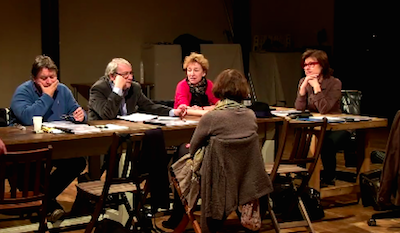
\includegraphics[height=3.3cm]{table_rehearsals}
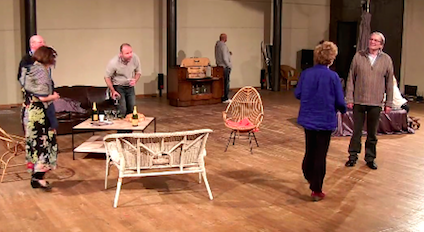
\includegraphics[height=3.3cm]{studio_rehearsals}
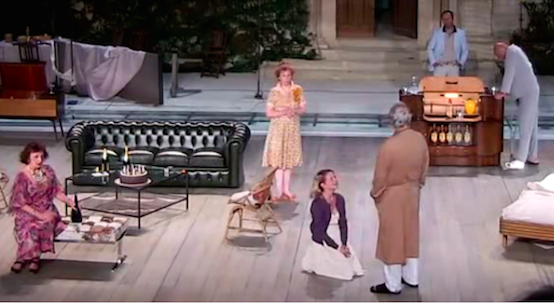
\includegraphics[height=3.3cm]{stage_rehearsals}
\caption{Three successive steps in the theater rehearsal process for \emph{Cat on a~hot tin roof}: (a)~Table readings; (b)~Early rehearsals in a~studio; (c)~Late rehearsals on stage (including dress rehearsals and technology rehearsals).}
\label{fig_rehearsals}
\end{figure*}


%%%%%%%%%%%%%%%%
\section{Introduction}
\label{sec:intro}

%\todo{0.5 pages (Rémi)}
%\todo{BE : Remarque générale :-attention à l’aspect Opéra : pas présent pour l’instant au moins dans le titre, l’introduction et la partie état de l’art… S’il faut gagner de la place, il faudra peut-être faire sans (simplement en mentionnant dans le papier le fait que le processus a également été appliqué sur de l’opéra mais que pour des raisons de place…) }

%\todo{0.5 pages (Remi)}

This paper presents the results of a~two-year research project dedicated to the creation of a~digital archive holding the complete rehearsals of two recent productions of a~theater play and an opera. To the best of our knowledge, this is the first time that exhaustive video recordings of theater and opera rehearsals are made available to researchers in the digital humanities at such a~large scale. Quoting from a~2007 DVD release%
\footnote{DVD \emph{In the Company of Actors}: \url{http://www.imdb.com/title/tt1059798/}}
of theater rehearsals, we acknowledge that  {\em ``within the world of theatre the rehearsal room is a~sacred space---the private domain where boundaries are pushed, risks are taken, mistakes made, vulnerabilities exposed and, at its very best, magic created. It is not a~place into which the public is often, if ever, invited.''} In our case, the directors of the theater and opera productions were a~leading force to open this sacred space---digitally.  This achievement was made possible by introducing a~specifically designed, non-intrusive workflow for a~natively digital archive from capture to editorialization, including collaborative annotation, audio and video processing, data modeling,  and hyperlinking, which we describe in the present paper.


%The French title of the project refers to the multiple timelines at work in this archive: all rehearsals timelines, from the first readings to the opening night, in addition to the storyline of the play. The title also refers to putting the video archive "online" ({\it i.e.} "en ligne") on the web. 


% (captation/annotation/enrichissement/publication/éditorialisation)}
%\todo{BE: quelle différence entre annotation et enrichissement ? --> je pense que seul "annotation" suffit)}

%The objective of the \emph{Spectacle en Ligne(s)} research project was to develop novel intuitive and interactive software tools to make it easier to  create and publish annotated video archives of theater performance and rehearsals. 

Archiving video recordings of live performances is important for preserving the cultural heritage of the performing arts but it is not yet a~common or systematic practice, and theater remains known as {\em the ephemeral art}~\cite{Reason06,Bouchez07}. This is likely to change in the near future, as high-quality video recording equipements are becoming more widely available to theaters.   Many organizations around the world now actively produce and archive video recordings of theater performances. The Theater on Film and Tape Archive (TOFT) provides research access to more than 20,000 video recordings of New York and regional theater productions since 1970.  The National Video Archive of Performance (NVAP) at the Victoria and Albert Museum London provides research access to video recordings of numerous renowned theater performances produced across the UK since 1992. 

Recently, such efforts have been extended to the World Wide Web. The start-up company Digital Theater 
creates video recordings of  theater productions  and makes them available  online for a~fraction of the cost of a~theater seat. The French National Institute of Audiovisual\footnote{French National Institute of Audiovisual: \url{http://www.ina.fr/}} (INA) allows viewers to download a~large number of   television broadcasts of historical theater performances. France Televisions' Nouvelles Ecritures\footnote{Nouvelles Ecritures is the new media department of France Televisions, producing and experimenting with new formats like webdoc, transmedia, virtual reality, \emph{etc.}: \url{http://nouvelles-ecritures.francetv.fr/}}  has been experimenting with an augmented theater experience for the Web,\footnote{Théâtre sans animaux: \url{http://nouvelles-ecritures.francetv.fr/theater-sans-animaux/}} showing five different versions of the same play \emph{Théâtre sans animaux}\footnote{\emph{Théâtre sans animaux} by Jean-Michel Ribes} at different stages of the production (including rehearsals) and presented in different styles. Theaters and operas also use the World Wide Web to share extracts and trailers of upcoming performances for publicity purposes. 

In most instances, performances are recorded with a~multi-camera, multi-take approach derived from broadcast television common practices. Having multiple viewpoints is especially beneficial for studying actor performances.  One extreme example is John Gielgud's  \emph{Hamlet} starring Richard Burton in 1964,  which used 19~cameras.  One problem with the ``multiple camera, multiple takes'' technique used by television broadcasters  is that it is costly and time-consuming to produce; and it generates huge volumes of data, which are  difficult to organize into an accessible and usable archive. Or more frequently, the rushes  are just ignored and only the edited version is kept as an archive. 

In this work, we take a~radically different approach, where we record the entire rehearsals from the same viewpoint.  As early as 1966, Jean-Luc Godard remarked: {\em ``Why do theater people never film their performances to keep  them as an archive? This would be very simple: put the camera in the middle of the orchestra seats with a~medium lens---not a~zoom lens---because it would already be making choices and propose an interpretation''}~\cite{Godard66}. Accordingly, our approach in this project has been to record the rehearsals from the director's viewpoint  with the highest possible video resolution, and to augment them with detailed, high-level  annotations that make it possible to quickly  search, browse, and even re-edit the archive interactively. 

%Which brings us back to Godard's citation. How can we create  an archive which is  more than an interpretation made by a television director and which is more than a video surveillance recording of the theater stage? 

%\todo{i believe this paper talks about something else than multiplying the points of view @Remi: need to be reformulated: "our approach in this paper..."}

%\todo{SHOW IMAGE OF THE CAMERA AND ROOM ?}

What we lose is the variety of viewpoints, which is typical for television broadcasts. What we gain is the ability to compare different versions, measure progress, and understand the rehearsal process by the virtue of having a~single spatial reference. We also experimented with state-of-the-art computer vision techniques for varying the framings and shot sizes interactively  by making use of a~{\em virtual}  zoom lens~\cite{Gandhi14,Gandhi15}, which makes it possible for researchers and amateurs alike to use the archive as {\em stock footage}, which they can re-frame and re-edit according to their own interpretation (this is described in Section~\ref{sec:scenarios}). 

As a~case study, the project has released an Open Data archive of the complete rehearsals of two performances played in 2013: \emph{(i)}~a~French translation and adaptation of \emph{Cat on a~hot tin roof} written by Tennessee Williams and directed by Claudia Stavisky, \emph{(ii)}~the baroque opera \emph{Elena}, composed by Francesco Cavalli, directed by Jean-Yves Ruf and conducted by Leonardo García Alarcón.


%In this paper, we describe our effort to create exhaustive video recordings of the complete rehearsals, rather than a single performance, of a theater play and publishing it online. This raises original and interesting scientific, technological, and social issues, and brought us to question the nature of the archive as a digital heritage through various prospective usages (see  Section~\ref{sec:scenarios}). 

The paper is organized as follows. Section~\ref{sec:stateoftheart} reviews previous work in using video as an archive for theater. Section~\ref{sec:context} describes the context of theater rehearsals and introduces the key concepts that govern the archive. Section~\ref{sec:workflow} describes the workflow that was created to produce, annotate, and publish the archive. Section~\ref{sec:scenarios} describes usage scenarios and applications that were developed to support access to the archive by different audiences. Section~\ref{sec:conclusion} concludes with limitations and future work.

%\todo{Make sure the paper structure is correctly described}


%%%%%%%%%%%%%%%%
\section{State of the art}
\label{sec:stateoftheart}

Audio and video recordings are useful resources in the field of performance studies~\cite{mcauley1994video,Bravo07} and rehearsal studies~\cite{McAuley06,McAuley08}. Yet, in practice, researchers have limited access to performances and must often refer to their own memories of the production or the rehearsals. Previous work on constituting video archives of rehearsals includes the work of Pascal Bouchez with Daniel Mesguich\cite{Bouchez07} and some clever use of multiple cameras and multiple takes edited together into high quality movies. Another notable exception is {\em In the company of actors}, a~documentary movie about a~production of \emph{Hedda Gabler} with Cate Blanchett in the title role~\cite{Darling07}. Even in those two cases, only an edited version (an interpretation)  of the rehearsals is made available to the public.


%RR removed those references . ~\cite{Selbourne82,Sher85,Stafford00,Stern00}.  

\paragraph*{Audio and video processing}
A useful feature for a~large video archive is the capability to retrieve video segments based on which actors 
are performing and which segment of the play script these actors are performing. In order to relieve annotators from the burden of precisely annotating which actors are present in which frames and speaking (or singing) which lines of the play script (or score),  we experimented with automatic audio and video processing methods. The topics of actor~\cite{Hilton06} and speaker~\cite{Miro12} recognition are very active in the audio and video processing research communities, but very little work has been dedicated to the special case of live performances. The stage is a~complex and cluttered environment  with complex lighting and vast dimensions, which makes automatic audio and video processing quite challenging. 

One approach to indexing multiple theater rehearsals and performances is to automatically align
all of them to the same play script. The {\em script-sync} feature in the Avid Media Composer editing suite
is a~well-known example of an off-the shelf solution for the alignment of video recordings with their scripts word-by-word. Such tools are based on Hidden Markov Models (HMM) and work by computing  a~forced alignment 
between the play script and the audio recording. Nevertheless they require very high quality 
sound recording and fail in the presence of music, reverberation and background noise. This makes them
unsuitable for our case. Speaker change detection (also called speaker diarization) is an alternative method
which provides line-by-line rather than word-by-word alignments and has been demonstrated 
on television shows~\cite{Sankar09} and theater recordings~\cite{Caillet13}. In Section~\ref{sec:scenarios},
we describe a~special-purpose speaker diarization method that we developed for aligning multiple versions 
of the same scene temporally using the common play script as a~pivot representation. In the case of music,
script-following methods could similarly be used to provide bar-by-bar alignments.

%Swedbeerg describes a system for localizing actors on a stage using RFID sensors carried by the actors~\cite{Swedberg}
%but their system is intrusive and costly, which severely limits its usefulness in practice.  Recent work in computer vision \cite{Dalal05,TapaswiBS12,Gandhi13} make it possible to detect and name actors in video automatically with minimal user input (example images) and we report on experiments in Section~\ref{sec:scenarios}). 

\paragraph*{Hypervideo and interactive documentaries}

The term \emph{hypervideo} is commonly used to refer to
\textit{``a~displayed video stream that contains embedded user-clickable anchors''}
and annotations~\cite{sawhney1996hypercafe}, %smith2002extensible 
allowing for navigation between the video and other hypermedia elements.
%In a~2006 article in \emph{The Economist}, the authors write 
%\textit{``[h]yperlinking video involves the use of `object-tracking' software
%to make filmed objects, such as cars, clickable as they move around.
%Viewers can then click on items of interest in a~video
%to watch a~related clip; after it has played,
%the original video resumes where it left off.
%To inform viewers that a~video is hyperlinked,
%editors can add highlights to moving images, use beeps as audible cues,
%or display still images from hyperlinked videos
%next to the clip that is currently playing''}~\cite{economist2006hypervideo}.
%\todo{PA: je trouve cette définition trop longue, trop détaillée, et franchement, dans un article scientifique, je pense qu'on serait aussi crédible avec une définition de nous qu'avec une définition de 'The Economist'. Je serai pour simplement reprendre l'idée de la phrase qui suit}
In standard literature, hypervideo is considered a~logical consequence
of the related concept of \emph{hypertext}~\cite{economist2006hypervideo}. %%bernerslee1990hypertext
In contrast to hypertext, hypervideo necessarily includes a~time component,
as content changes over time.
Therefore hypervideo has other technical and aesthetic requirements
than hypertext, the most obvious one being appropriate segmentation in scenes
or even objects.
The opportunities for feature-rich semantic hypervideos are endless,
only limited by feasibility and ease of their creation.
In this paper, we share our approach to affordably and practically document
the creation of theater and opera productions with video and Web technologies.


%%%%%%%%%%%%%%%%
\section{The rehearsal process}
\label{sec:context}
%
%\todo{Contexte de l'archive (1 page - Nicolas)}
%\todo{du terrain à la donnée: ce qui nous a amené à structurer les données de cette façon}
%\todo{description des besoins}
%\todo{Actors and participants:  theater rehearsals involve many actors and participants, not limited to actors in the play.}
%\todo{Other participants include the director and her assistants, the lighting director, the sound director, the stage manager, technicians, etc.}
%\todo{Performances}
%\todo{Discussions}

Live performance rehearsals involve many actors and participants, not limited to theater actors,  including the director and  directing assistants, singers and musicians, lighting directors, sound directors, stage managers, technicians, \emph{etc.} The archive and its metadata were designed to take all of them into account, based on a~careful analysis of the experimental fields of  theater and opera.

%The the descriptions rely strongly on the chosen fields of study (\todo{what's the proper translation for terrain d'études ? PA: field of study me parait bien: \url{http://www.linguee.fr/francais-anglais/traduction/terrain+d'étude.html}}), \emph{i.e.}, in our case the rehearsals of the play and the opera themselves, but more importantly the methodologies of the creative crew.

%\subsection{theater and opera as experimental fields}

Theater and opera turned out to be distinct experimental fields with important differences in the rehearsal process.  The two experiments in our case were original productions of  Tennessee Williams' \emph{Chatte sur un toit brûlant} and Francesco Cavalli's \emph{Elena}. Both of them  were rehearsed during spring and summer of 2013, in a~period of eight and six weeks respectively. The project was about documenting the entire rehearsal process, from the first \emph{table readings}, where actors read the script together for the first time, all the way to the \emph{opening night} (see Fig.\ref{fig_rehearsals}). However, the nature of the creative work diverges considerably from the \emph{mise en scene} of a~contemporary play to an ancient and obscure baroque opera, musically updated with a~consequent adaptation work. Those aspects motivated us to design  
a generic system that could be deployed in such different contexts.

\subsection{The rehearsal process}

A~performance rehearsal is a~closed-door privileged moment where actors and director work in a~protective intimacy that allows them a~total commitment to their art. The idea of filming those moments of intimacy, moreover exhaustively, could cause discomfort at best, or even rejection at worst, from professionals considering as sacred the privacy of rehearsal. This aspect was taken into account in the design of the system, 
which was engineered to be minimally intrusive and maximally respectful of  the creative process at work
during the rehearsals.

\begin{figure}[htb!]
  \centering
  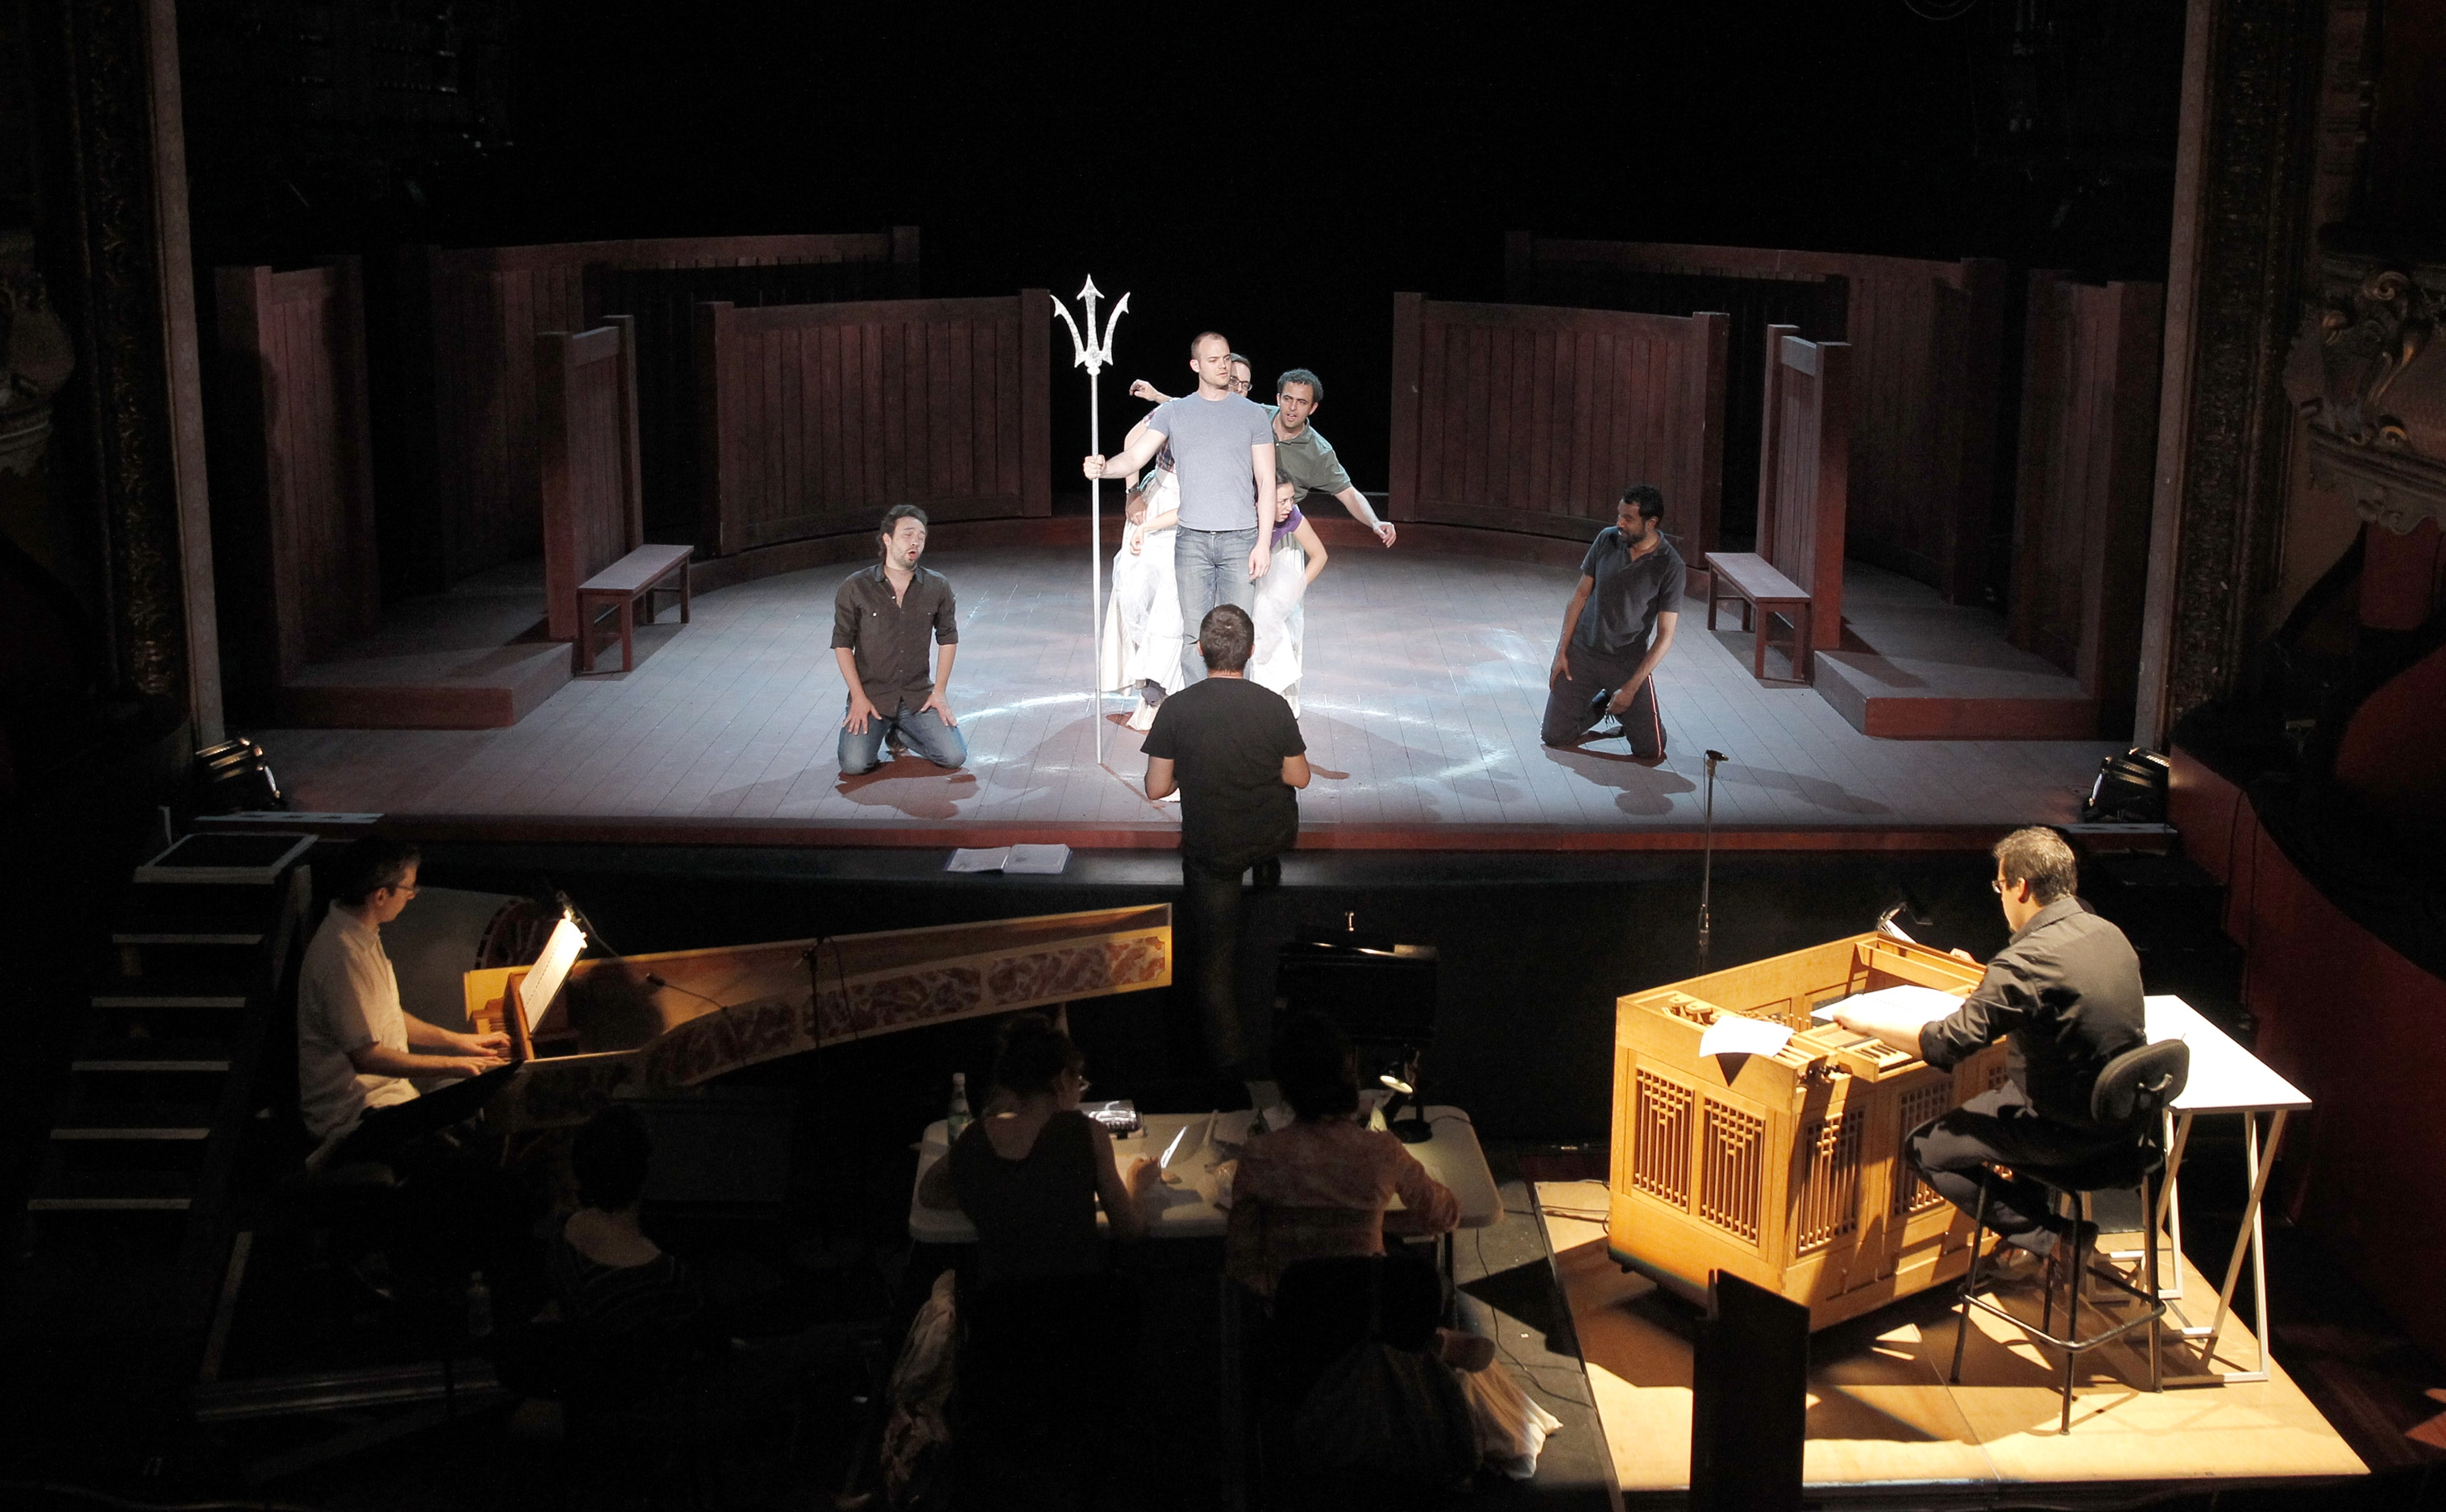
\includegraphics[width=\columnwidth]{elena}
  \caption{Rehearsal of the opera \emph{Elena}, Festival d’Aix-en-Provence, 2013. © by Pascal Victor / Artcomart.}
  \label{fig:elena}
\end{figure}


\subsection{Performances and discussions}

The rehearsals unfold according to a~relatively classic \emph{modus operandi}: the acting and directing crew gathered daily in a~studio room or on stage to work through certain parts of the script or of the partition. Based on observations of previous rehearsals by the same director, we were able to identify a~recurring pattern in the rehearsal process: an alternation of performances during which actors play their roles, and discussions during which the actors and the director interrupt the performance and make comments and suggestions. This alternation of performance and discussion became a~central element of the data model used to annotate the archive. We reckon that a~director working according to a~different methodology would have generated a~very different corpus and annotation set.

%%BE ce qui suit n'est pas nécessaire je pense (déjà présent section Annotation)
%\todo{BE: déjà dit un peu plus loin (section Annotation)}
%Usual information (\emph{i.e.} metadata) coming from the fields of theater and opera were integrated to describe the working session---with or without set, costume, lights, sound effects, music, orchestra, \emph{etc.}, but also the presence of the actors on stage and the precise text reference.
%%Fin BE
%
%\subsection{Text and partition reference}
%\todo{BE: est-ce que cette sous-section est nécessaire? Quel est son contenu ?}
%\todo{[...]}
%

%%%%%%%%%%%%%%%%
\section{Archive construction and publication workflow}
\label{sec:workflow}

%\todo{(2,5 pages)}
%\todo{complete workflow of construction and publication process}

Digital heritage projects often focus on digitalization of analog materials and data,
when others would focus on the usage and the valorization of digitalized resources.
In our case, a~specific feature of the project was the design decision to create a~natively 
digital archive from scratch,  taking into account its potential usages by different audiences.
We therefore built a~complete pipeline from the design and the making of the archive
to its publication and usage scenarios. This section describes the details of the workflow 
and describes all the hardware and software components that enabled  the construction 
and the publication  of the archive.

\subsection{Video recording}
%Non intrusive, push-button, integral, full HD, sound
%\todo{BE - remarque générale: je préfère le terme annotation au terme index}
In the context described previously, the video recording required a~non-intrusive and easy setup for non-technical operators. Actually, their profile must belong to dramaturgy and performing art in order to dedicate their attention to performance and directing description. Therefore, the apparatus was designed to be fully \emph{plug\ \& play} with a~single record button to start a~capture session.
The collected corpus embraces the integrality of the rehearsals, from the ``text walk-through'' at the table to the final dress rehearsal, with about five to seven working hours a~day, which in consequence result in likewise five to seven hours of recorded and annotated video every day.

The unit for video recording and annotating is typically composed of a~PC laptop that is connected to a~video camera mounted on a~tripod and remotely controlled from the PC, of an omnidirectional microphone as input of a~small sound mixing desk, in turn linked to the laptop. This system can be easily set up and wrapped up, is movable, and can fit in a~studio room without burdens. Running on a~dedicated Linux distribution, the unit executes and displays only one software: an interface through which the operator can \emph{(i)}~remotely control the camera and \emph{(ii)}~take notes synchronously. 
The technical specifications of the original video files are the format \texttt{.mkv}, the codec H264, and the resolution of $1920 \times 1080$ pixels (full HD).

%\begin{figure}[htb!]
%  \centering
%  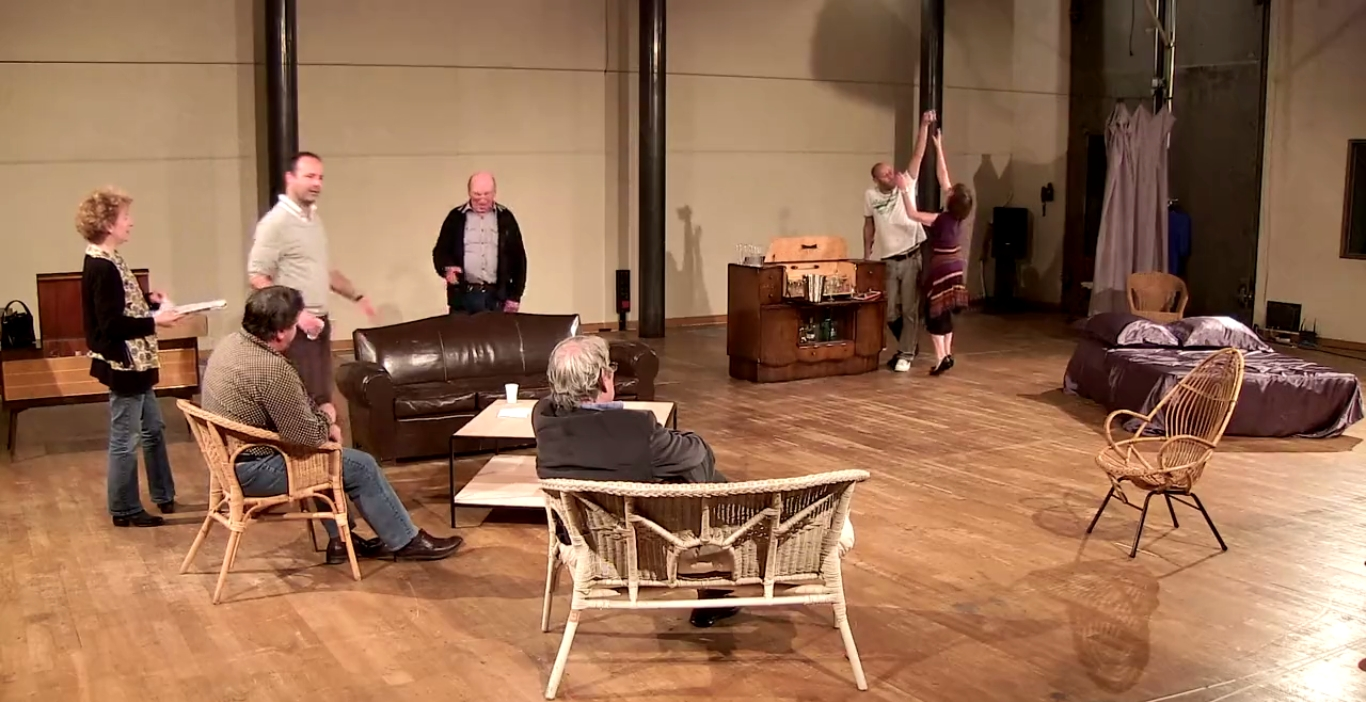
\includegraphics[width=\columnwidth]{onstudio}
%  \caption{Studio rehearsal of \emph{Chatte sur un toit brûlant} in Paris}
%  \label{fig:onstudio}
%\end{figure}

\subsection{Annotation}
%\todo{attention à l'homogénéité du vocabulaire: annotations; metadata; data}
Simultaneously to the live video capture, the operator was asked to describe the rehearsals in his own words using  the note-taking tool. The data produced during this annotation process were synchronized with the video stream and encoded into an XML format based on the Cinélab data model.\footnote{Cinélab Data Model: \url{http://liris.cnrs.fr/advene/cinelab/}}

Annotations of the  rehearsals were further classified  into two main categories: descriptions and interpretations.  Description annotations contain contextual and objective information about the rehearsals  (performances and  discussions, with or without costumes, time, location, \emph{etc.}), whereas interpretation annotations targeted the dramaturgy and aesthetics of the performances themselves---with free observations and comments on the creative work. The interpretations were further classified into sub-categories. Those sub-categories (see tables~\ref{table:categories1} and~\ref{table:categories2}) emerged progressively along the rehearsal process according to the point of view and the focus of the operator. 
In contrast, different categories emerged for theater and opera, reflecting both the different nature of these performing arts, and the personal point of view of each annotator.

\begin{table}
\small
\begin{tabular}{|p{2.8cm}|p{1.8cm}|p{1.2cm}|p{1.2cm}|}
\hline 
  & Cat on a~Hot Tin Roof  & Elena & Total \\ 
\hline 
Number of videos & 70 & 100 & 170 \\ 
\hline 
Total duration (h) & 242 & 177 & 419 \\ 
\hline 
Total volume (TB) & 2.47 & 1.60 & 4.07 \\ 
\hline 
Annotations & 3,530 & 6,968 & 10,498\\ 
\hline
\end{tabular} 
\caption{Size of the video corpus}
\label{table_facts}
\end{table}

The result of this synchronous annotation was an augmented  video stream with semantic metadata, also considered as intra-video indices, making the video corpus easily searchable with a~proper search engine.

\subsubsection{Data model} Figure~\ref{fig_data_model} describes the main elements of the data model used by the note-taking tool. This model results from a~workshop analysis, gathering several kinds of attendees (researchers, producers, dramatists, film editors)---each kind having different requirements concerning rehearsals annotation capabilities. It focuses on annotations that have to be created in realtime (\emph{i.e.}, during the rehearsal). \newline

A session annotation is linked with a~video file and represents a~rehearsal session (typically lasting a~half or full day). A~session annotation is connected to a~place (where the rehearsal takes place) and to a~creation (linked to a~work and castings). A~session annotation is made up of chapters that represent performance or discussion times. A~chapter contains contextual metadata (\emph{i.e.}, with or without costumes, lights, sets and musical inserts) and includes a~direct reference to the section of the work being performed or discussed (for theater, we used page and line numbers in the play-script; for opera, we used page and bar numbers in the musical score). 

%Chapters also may contain categorized moments of interest. 

%\todo{PA: j'ai remplacé la parenthèse ``so-called categories'' et rajouté l'adjectif ``categorized'', car la parenthèse me semblait un contre-sens: les moments d'intérêt ne \emph{sont pas} des catégories}

\begin{figure*}[ht]
\centering
{
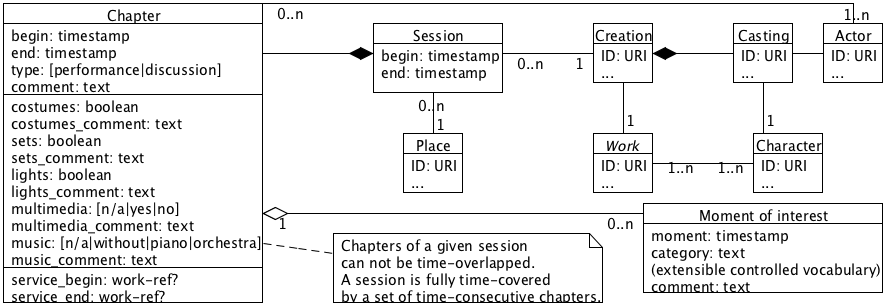
\includegraphics[width=0.8\linewidth]{UMLet_Data_modelvFullPage}
\caption{Main elements of the data model used by the note-taking tool}
\label{fig_data_model}
}
\end{figure*}


\subsubsection{Practical usage of the model} Generally speaking, at the beginning of a~rehearsals caption process for a~given work, an operator first enters some time-stable data in the note-taking tool: the creation, work, actors, characters, rehearsals place. Additional data can next be entered or updated during a~rehearsal session---\emph{e.g.}, contextual data (costumes, sets, \emph{etc.}) about a~given chapter (inherited from a~previous one, if any).
%BE on peut pour gagner de la place juste mettre les éléments Session, Chapter, Moment of interest..

\subsubsection{Annotation categories}
%\todo{BE Proposition titre subsubsection: Emerged categories review}
%\todo{Emerged categories: je voulais dire, les catégories qui ont émergées lors de l'annotation. Je tente "inherited", est ce que cela convient ? Pas tout à fait clair non plus.}

The annotation process revealed a~rich set of categories associated to interpretation annotations, reflecting 
the  specific domains of theater and opera and the personal viewpoint of the annotator. Tables~\ref{table:categories1} and~\ref{table:categories2} present the richness of these categories and the potential of the archive for further research on genetic analysis of creative works.

\begin{table}
\centering
\small
\begin{tabular}{|p{6cm}|r|}
\hline 
Category & Occurrences \\ 
\hline 
alternative performance proposition & 70 \\ 
\hline 
conflict & 7 \\ 
\hline 
decision & 14 \\ 
\hline 
detecting an issue & 81 \\ 
\hline 
doubts & 23 \\ 
\hline 
improvisation & 16 \\ 
\hline 
intervention of the director & 554 \\ 
\hline 
intervention of the first assistant & 3 \\ 
\hline 
intervention of the technical staff & 22 \\ 
\hline 
opinion of an actor & 26 \\ 
\hline 
performance of an actor & 331 \\ 
\hline 
questioning & 4 \\ 
\hline 
reference to real world & 3 \\ 
\hline 
rehearsal with text & 1 \\ 
\hline 
repeating a~scene & 451 \\ 
\hline 
request from an actor & 62 \\ 
\hline 
run-through & 42 \\ 
\hline 
script adaptation & 6 \\ 
\hline 
space issue & 6 \\ 
\hline 
\end{tabular}
\caption{Annotation categories and number of occurrences for the theater play \emph{Chatte sur un toit brûlant}}
\label{table:categories1}
\end{table}
%\todo{mise en forme des captions pour les tableaux > why capitals letter ?} 

\begin{table}
\centering
\small
\begin{tabular}{|p{6cm}|r|}
\hline 
Category & Occurrences \\ 
\hline 
accessories & 292 \\ 
\hline 
address & 247 \\ 
\hline 
articulation & 357 \\ 
\hline 
breathing & 25 \\ 
\hline 
character definition & 725 \\ 
\hline 
characters relation & 820 \\ 
\hline 
conflict & 27 \\ 
\hline 
cooperation director/conductor & 178 \\ 
\hline 
costumes & 711 \\ 
\hline 
decision & 154 \\ 
\hline 
decoration & 14 \\ 
\hline 
emotion & 134 \\ 
\hline 
gestures & 346 \\ 
\hline 
improvisation & 52 \\ 
\hline 
instrumentation & 118 \\ 
\hline 
intonation & 65 \\ 
\hline 
lights & 221 \\ 
\hline 
moving & 830 \\ 
\hline 
music dynamics & 158 \\ 
\hline 
partition modification & 166 \\ 
\hline 
phrasing & 131 \\ 
\hline 
power relation & 47 \\ 
\hline 
pronunciation & 109 \\ 
\hline 
reference to camera & 1 \\ 
\hline 
research & 327 \\ 
\hline 
scenery setting & 85 \\ 
\hline 
seduction relation & 66 \\ 
\hline 
tempo & 406 \\ 
\hline 
voice ``color'' & 112 \\ 
\hline 
working on the text & 104 \\ 
\hline 
\end{tabular} 
\caption{Annotation categories and number of occurrences for the opera \emph{Elena}}
\label{table:categories2}
\end{table}  
 
\subsection{Data cleansing and conforming}
%\todo{(nicolas)}
%\todo{@Remi: conformation est un terme anglais. Je l'explicite dans la partie ci-dessous. Je pense que cela sera compréhensible. PA: et pourquoi pas 'curation' qui est peut-être mieux compris dans le milieu du digital heritage, et également employé pour les données ??}
After the rehearsals, we centralized the data on a~server for video encoding and annotation metadata conformation. Due to the tight agenda of the project, the annotation software did not implement a~strict certification on data input. Therefore, as a~preliminary step before the ingestion of the corpus into the applicative platform, manual cleansing and conforming were executed on both the data (checking audio and video quality) and the metadata (merging similar categories, harmonizing the text reference format, correcting misspellings).

\subsection{Audio and video processing}
As an optional step, we trained statistical models of the actors' voices and appearances to detect and recognize them in the audio and video modalities. As explained later, this offers additional searching, browsing, and editing capabilities to our system, at the expense of (widely) increased processing time.

\subsubsection{Learning actor voices and appearances}
We used the ALIZE speech recognition system ~\cite{Bonastre05} for learning statistical models of each actor's voice from one example per actor. Each example is typically a~ten-second extended speech line recorded during the first reading of the play. In parallel, we trained statistical models of each actor's visual appearance, using example images from at least eight views~\cite{Gandhi13}. Examples are typically extracted from the first dress rehearsal, as the appearance models are dependent on costumes.  Those models can then be used to automatically align each performance with the play script and to localize actors on stage and on screen in all subsequent dress and tech rehearsals. 

\subsubsection{Alignment between play script and performances}

Using the ALIZE speech recognition toolkit, we built a~play-script following algorithm where rehearsals are assumed to be generated by a~probabilistic generative model.  More specifically, each  line in the play script is a~state in a~semi-Markov model with a~duration probability and a~speaker voice probability. In our experiments, this methods outperformed state-of-the-art speaker diarization methods based on HMM, which do not have duration models. % ADD THIS REFERENCE IF ACCEPTED FOR PUBLICATION \cite{Migniot15}. 
 

%\begin{figure}[tp]
%\centering
% 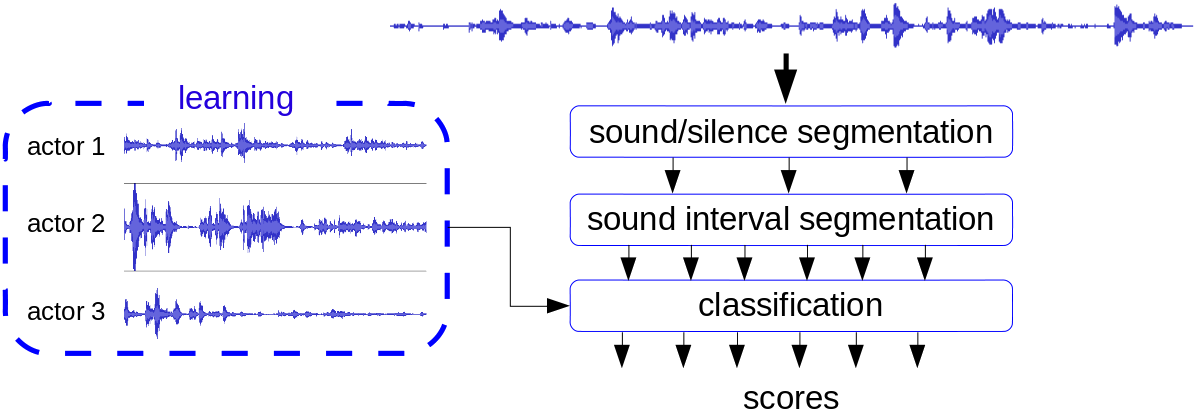
\includegraphics[width=\columnwidth]{diarizationT.png}
%\caption{In the speaker diarization phase, we learn a model of each actor's voice.
%They are used as observation probabilities in our Semi-Markov model of the rehearsals.}
%\label{fig_diarization}
%\end{figure}


\subsubsection{Actor detection and recognition} 

In some selected scenes, we  detected all actors present on stage in parallel based on their appearances
using a~method described elsewhere~\cite{Gandhi13}. Despite the challenging environment, this method provided very good results for  all actors in all tested sequences, where generic state-of-the-art tracking methods quickly drifted away from the target and were unstable both in presence of occlusion and fast movements. One drawback with the method is its computational cost, which made it impossible to perform
actor detection and recognition on the entire archive. Selected scenes were chosen for evaluation and validation purposes.

%%Based on their appearance model, we separately detect all actors present on stage. The qualitative results on this sequence are presented in Figure~\ref{fig_tracking_coahtr}. This example is particularly challenging  because of the fast displacements of the actors and the frequent occlusions between actors. Despite the challenging environment, our method provides very good results for the tracking of the six actors, where generic state-of-the-art tracking methods quickly drifted away from the target and were unstable both in presence of occlusion and fast movements \cite{Gandhi13,Migniot15}.
%%
%%\begin{figure}[tp]
%%\centering
%%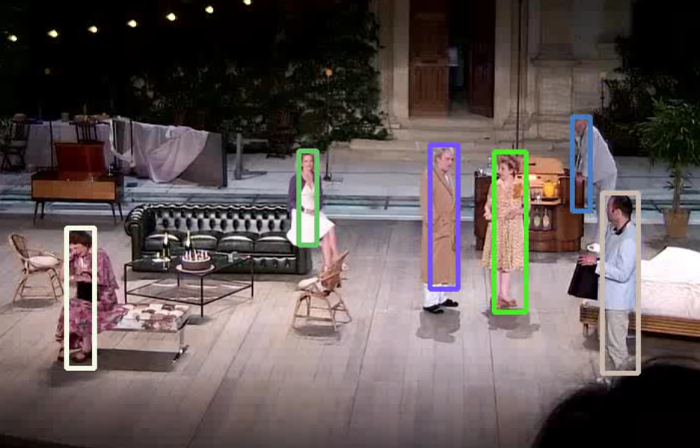
\includegraphics[width=\columnwidth]{tracking_coahtr}
%%\caption{Tracking of  the six characters of sequence $\mathcal{S}_4$. Using actors-specific detections gives an additional advantage in resolving multiple actor tracking.}
%%\label{fig_tracking_coahtr}
%%\end{figure}

 
%\todo{BE: Idem: Rémi, vous avez pas une réf. à vous à mettre là-dessus du coup ?}

%\cite{Nummiaro2002,Ross2008}  \cite{Kwon2010,Babenko2009} also drifted away with heavy occlusions.  \cite{Wang2011} failed because of large appearance changes and occlusions. Only our algorithm maintains its performance in this challenging example.


\subsection{Data publishing}
The project built on the applicative platform \emph{Ligne de temps}\footnote{Ligne de temps: \url{http://www.iri.centrepompidou.fr/outils/lignes-de-temps/}} to implement specific modules dedicated to fine-indexed, annotated video archives of performance rehearsals. \emph{Ligne de temps} is originally a~software designed for video annotation and indexation, inspired by the timelines usually used in video editing softwares, and was conceived for advanced film critique or pedagogy. It evolved into a~Web platform with Web player and front-end annotations modules. For the purpose of the project, \emph{Ligne de temps} was adapted to embed and display annotated video of performance rehearsals, taking into consideration the particular metadata and their potential usages.

\subsubsection{Ingest}
The ingest operation was made possible due to the previous step of data cleansing and conforming. It involved automatic referencing of the video files as media contents into the platform and the synchronization of the metadata (annotations) to the media contents. \emph{Ligne de temps} provides an applicative environment to search, consult, edit, and publish the media contents and their metadata, therefore bringing the rehearsal annotation data from static to dynamic. However, theater and opera archives were separated in two distinct access points, due to usage scenarios and to differences in data format.

% BE: Difference in data format. Le format reste pour moi le même (XML ici), le modèle aussi à peu de chose près (i.e. référence à un texte pour le théâtre, référence à une partition pour l'opéra, ce qui change un peu le modèle). Par contre, le contenu des données change (i.e. les catégories, par ex.). Du coup je ne sais pas si ça vaut le coup de mettre "differences in data format", je pense que "usage scenarios" suffit...
% Indeed, the search engine and further applications require a stable model of data to offer optimized user experience.
%\todo{BE remarque: supprimer cette phrase (stable model of data), cf. commentaires dans le source.}
% BE Du coup cette phrase est à supprimer de mon point de vue.

\subsubsection{Search engine}
%\todo{Write}
A faceted search engine was designed to perform complex requests on the archive based on available metadata.
Figure~\ref{fig:searchengine} displays the search interface for theater, divided vertically in two parts for different types of search operations:
\emph{(i)}~left side: searching chapters by rehearsal context data such as date of rehearsal, character(s) on stage, lines of the script, type of chapters, \emph{etc.}, providing a~sortable list of chapters,
\emph{(ii)}~right side: searching interpretation annotations by full text and/or by a~closed list of categories, providing a~sortable list of annotations. Thanks to the synchronization of metadata to the video stream, a~search result list from either side can be used as a~request to the opposite side. For instance, from the result list of annotations (right side), it is possible to extract all chapters with corresponding timecode (left side).

\begin{figure}[htb!]
  \centering
  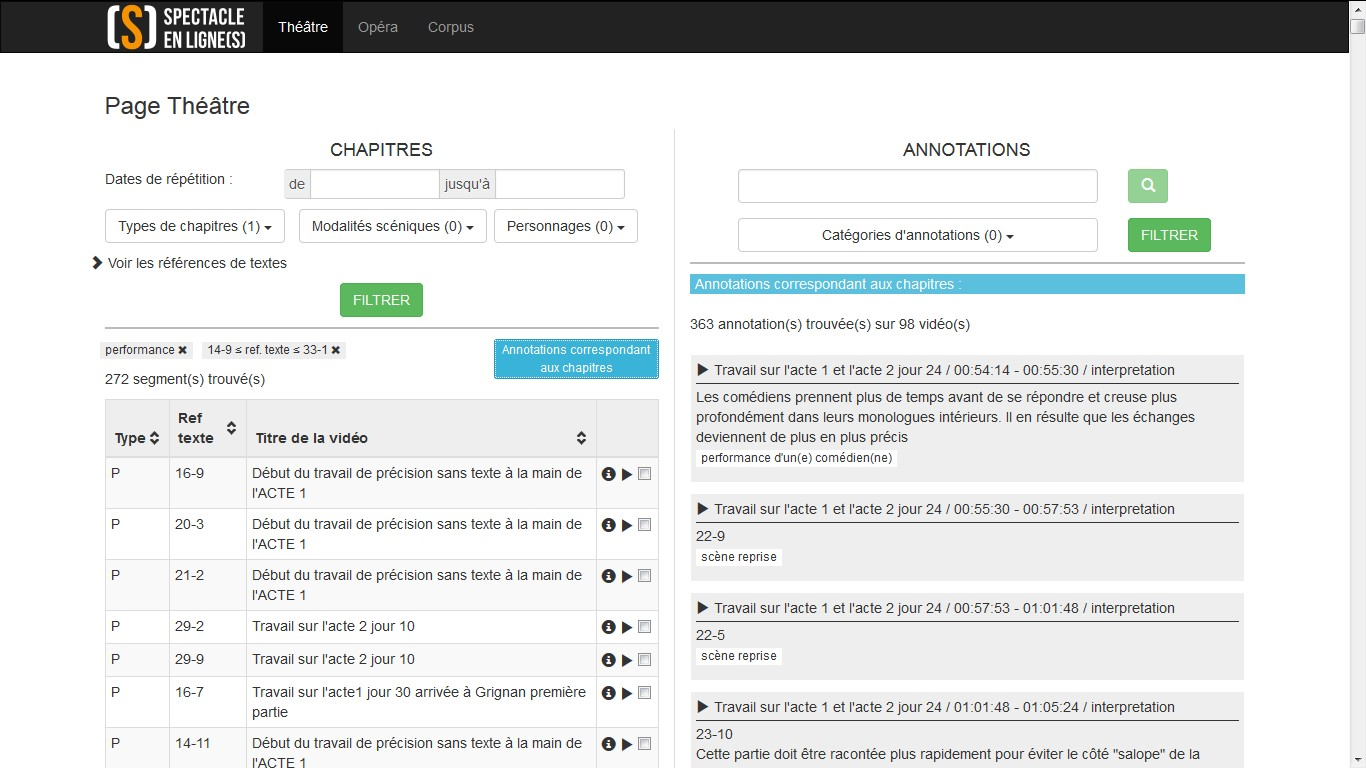
\includegraphics[width=\columnwidth]{searchengine}
  \caption{Multi-faceted search engine giving access to all archive materials. 
  Returned video segments can be watched and navigated as hypervideos.}  %for the theater archive
%    \todo{PA: j'ai viré les marges de l'image pour la rendre plus lisible, mais c'est encore très petit...}}
  \label{fig:searchengine}
\end{figure}


%\subsubsection{Metadata player}
%The \emph{Metadata player} is a front-end Javascript module articulating a HTML5 video player with time-stamped metadata displayed on a timeline representation. It communicates with \emph{Ligne de temps} to retrieve the synchronized metadata for each media content to be displayed. For the usage of the project, a dedicated player was designed to display the contextual chapters and the interpretation annotations on timelines and to provide the play script synchronized along the video, according to the text reference metadata.

%\begin{figure}[htb!]
%  \centering
%  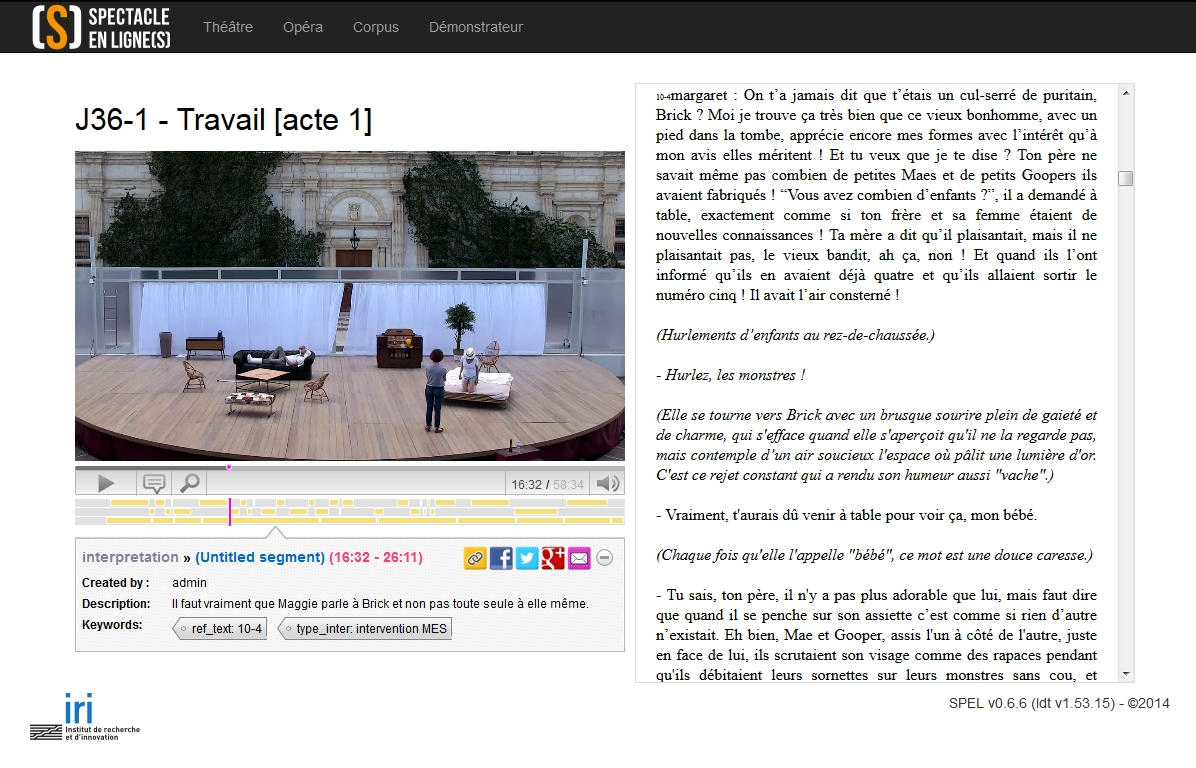
\includegraphics[width=\columnwidth]{mdplayer}
%  \caption{the Metadata player: video player augmented with synchronized play script and metadata (annotations)}
%  \label{fig:mdplayer}
%\end{figure}

\subsection{Linked Open Data compatibility}
In order to foster and ease multiple uses of the corpus,
it was important to make the collected information as accessible as possible.
For this purpose, we chose to comply with the principles of Linked Open Data~\cite{bernerslee2006linkeddata}.
This implied that every piece of information was both identified by and accessible at a~given URI, and that it 
was published using the RDF data model~\cite{cyganiak2014rdf11concepts}.

The Cinélab data model maps nicely into RDF, thanks to additional standards such as Media Fragments URIs~\cite{troncy2012mediafragments} that are used to precisely anchor annotations to video temporal fragments. Furthermore, Linked Data has the common query language SPARQL~\cite{prudhommeaux2008sparql}, so building new services on top of our corpus can be achieved with relative ease by reusing standard components. Finally, we used an approach called Linked Data Fragments, proposed by Verborgh \emph{et al.}~\cite{verborgh2014querying}, to make the data widely
available while preserving scalability.

But the benefit of Linked Data does not only lie in standardization. As its name implies, the key feature of this approach is to allow linking data across different sources on the Web, in order to combine it into otherwise inaccessible information. In the context of Digital Heritage, this notion is central, as data is often scattered in multiple institutions. While Linked Data is already widely used for museums or libraries,\footnote{
See, \emph{e.g.}, \url{http://data.europeana.eu/} or \url{http://data.bnf.fr/}}
its use with video has emerged more recently~\cite{vandeursen2012mediafragmentannotations,steiner2014webvtt},
and as far as we can tell, has not yet been widely considered for live performance archives.


%%%%%%%%%%%%%%%%
\section{Usage scenarios}
\label{sec:scenarios}
%\todo{(1,5 pages)}
In parallel to the design and implementation of the previously described workflow, the project anticipated several usage scenarios of the archive, taking into consideration the potential needs of future users. A~particular effort was made to address specific audiences with pedagogical scenarios, culture mediation scenarios, but also research and amateur scenarios. Some of these scenarios were implemented into demonstrators, others into mock-ups, allowing the partners of the project to freely explore prospective scenarios according to their interests. This prospective work was indeed central in the design of the continuous workflow in order to articulate the newly constructed archive with existing or prospective usages. This approach is one of the particularities of this project regarding researches in the digital heritage, \emph{i.e.}, to have considered the archive as a~living cultural object, even though the archive did not exist yet.

\subsection{Quantitative and qualitative analysis}
The massive aspect of the archive makes it difficult to apprehend. Both the nature of the archive, \emph{i.e.}, video as a~temporal object\cite{stiegler98}  and its total duration (419 hours for 170 video files) as well as the amount of annotations (10,498) demanded a~comprehensive and cognitively acceptable representation. Taking the project's title literally:
%\emph{Spectacle en ligne(s)},
\todo{anonymized (native language)}, \emph{i.e.},
%\emph{Performance in line(s)},
\todo{anonymized (translated)},
the archive can be viewed as multiple lines of rehearsals. We imagined a~matrix where the columns are pages in the play-script  (or the musical score) and the rows are days of rehearsal. The result is the distribution of the rehearsals according to the script or score over time.

%\todo{Remarque BE: illustration matrice sur théâtre plutôt qu'opéra (Elena), surtout si dans un futur proche il faut se concentrer sur le théâtre pour gagner de la place.. 
%NS: malheureusement, cette matrice est beaucoup plus détaillée et pertinente. Dans un sens, ça n'est pas très grave d'alterner opéra et théatre à mon avis.  RR: Can we show the matrices for both opera and theater ? The comparison is in itself interesting ! (and we can skip the ideal matrix)}

\begin{figure}[htb!]
  \centering
  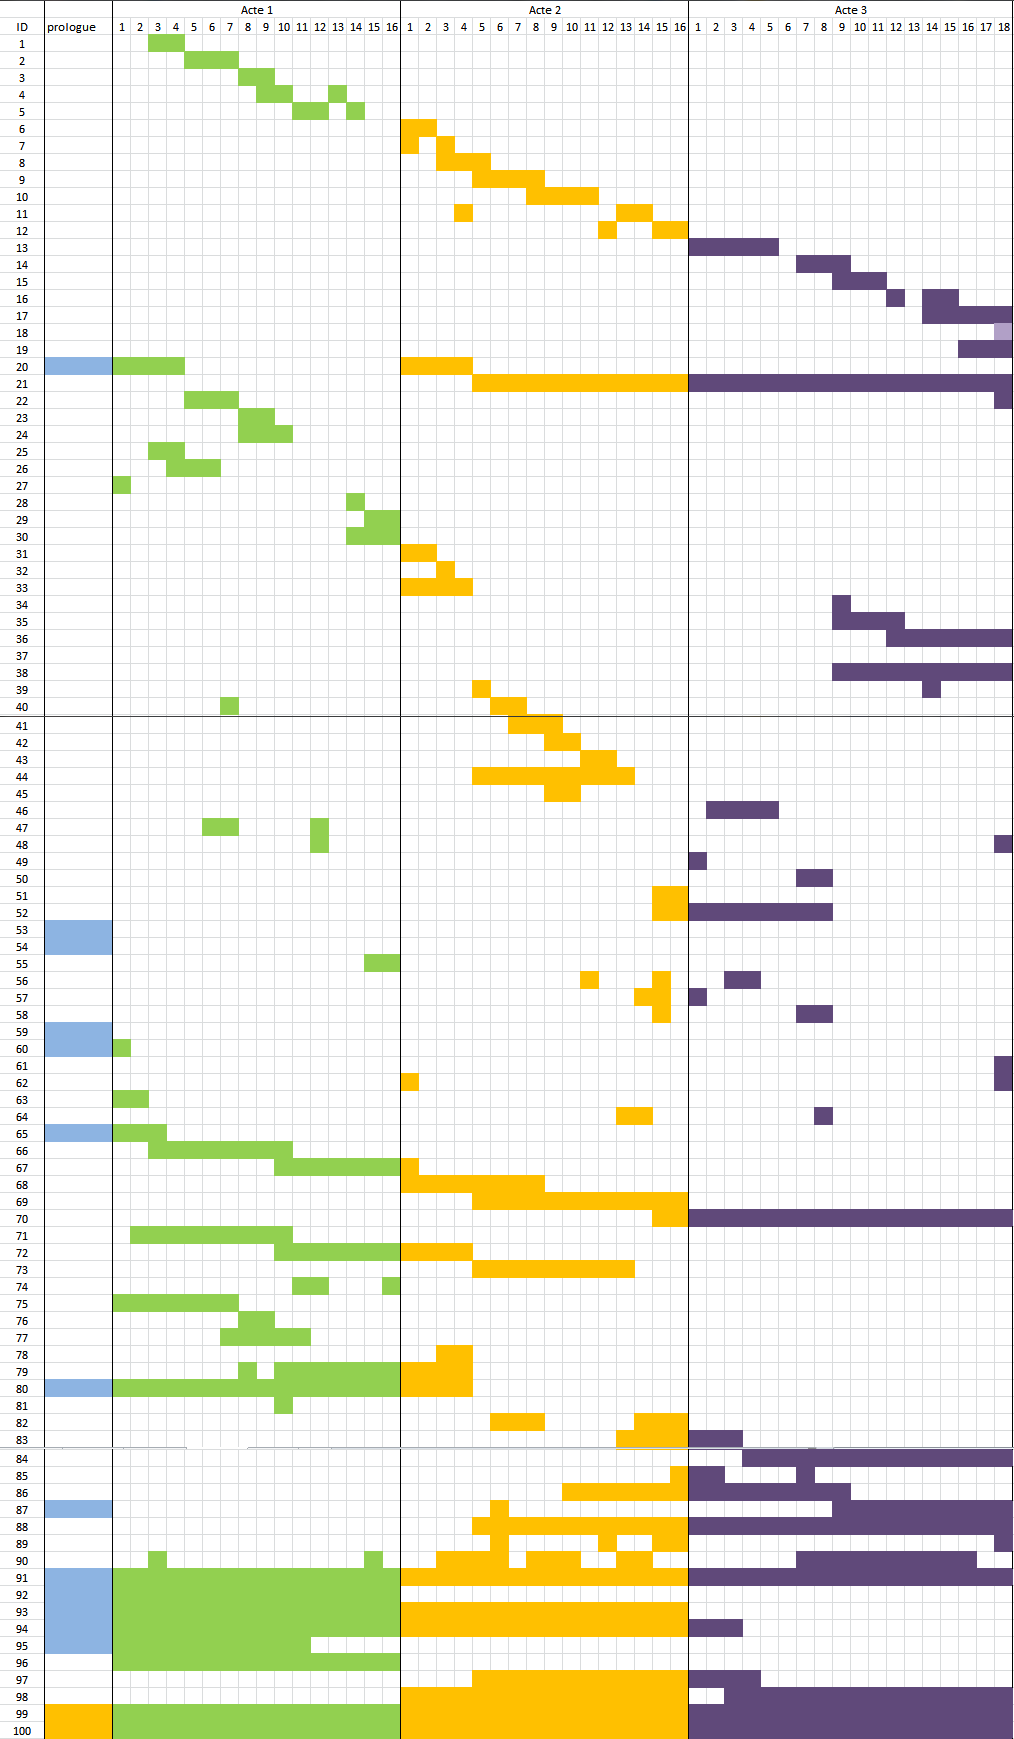
\includegraphics[width=\columnwidth]{elenamatrix}
  \caption{Matrix of distribution of the rehearsals according to the score of \emph{Elena} over time.} 
  %\todo{Explain what the colors mean}
  \label{fig:elenamatrix}
\end{figure}

%When audio processing was available, we were able to increase the granularity of the analysis to individual lines of the play-script. Similar capabilities could be added for opera rehearsals by using script-following technologies in future work.

%The figure models this idealistic representation.
%
%\todo{Remarque BE: je trouve que la figure du modèle de la matrice n'est pas super importante, à supprimer je pense si besoin de place. PA: je suis d'accord}
%
%\begin{figure}[htb!]
%  \centering
%  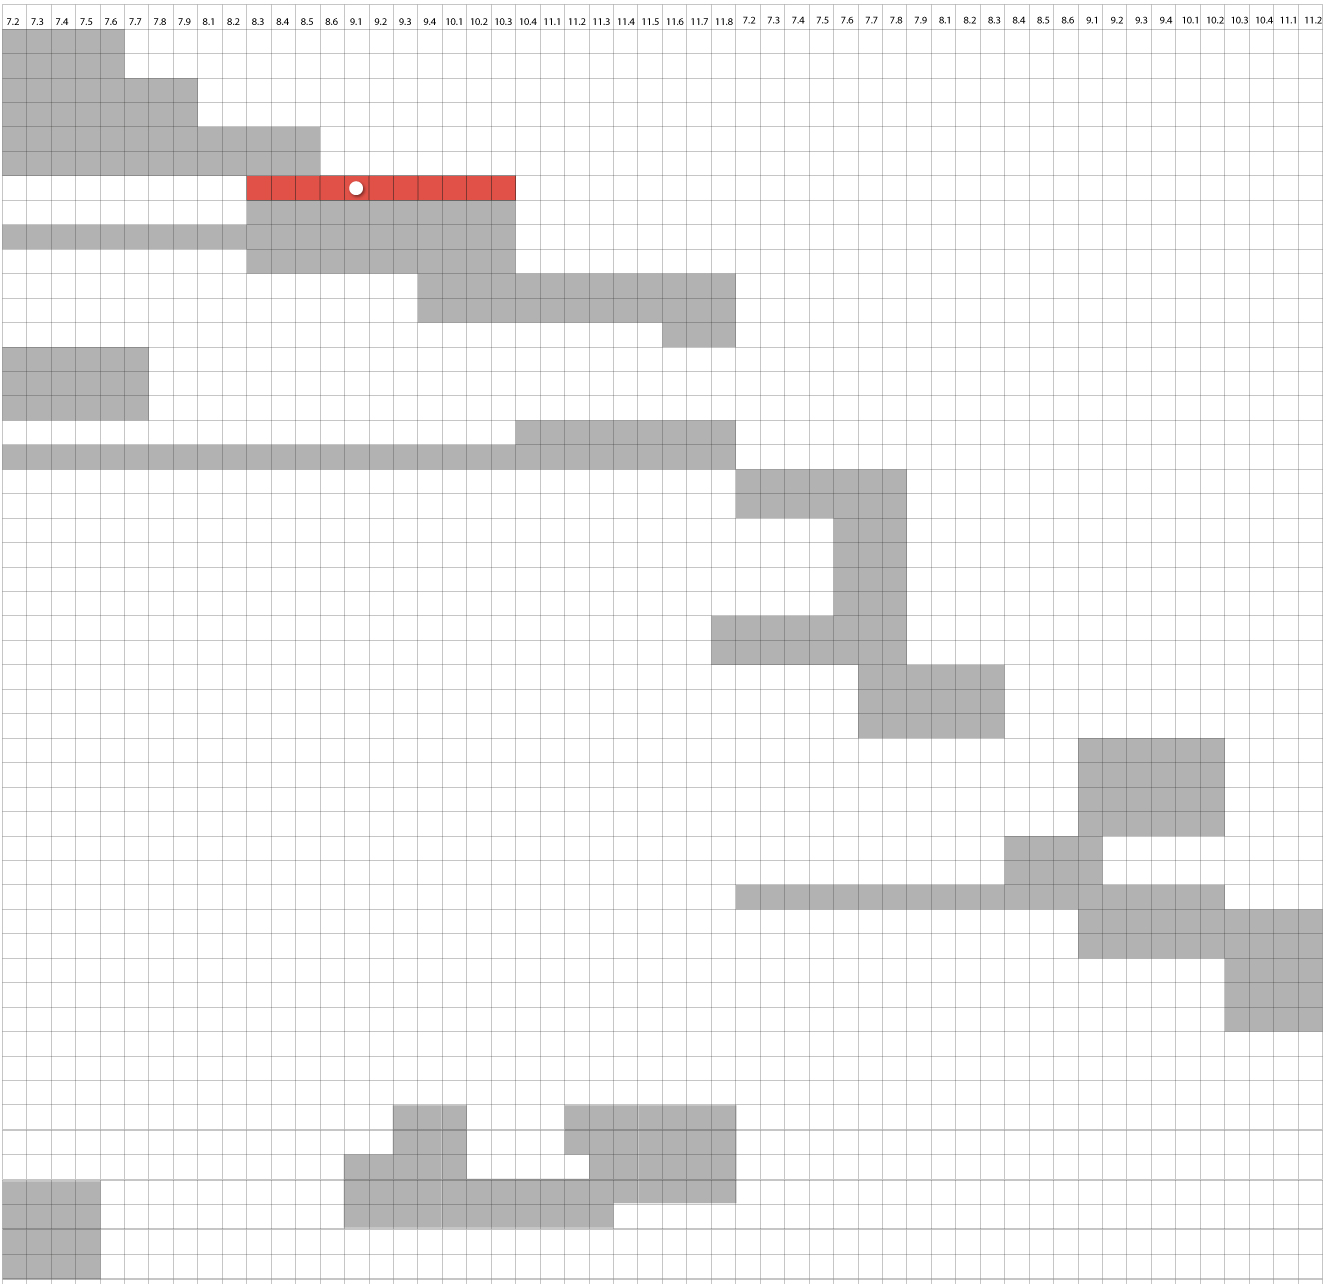
\includegraphics[width=\columnwidth]{fullmatrix}
%  \caption{Model of the matrix of distribution of the rehearsals over time with 1 unit = 1 cue in abscissa and 1 unit = 1 performance in ordinate}
%  \label{fig:fullmatrix}
%\end{figure}

%Such a representation achieves the initial objective of providing a comprehensive visualization suitable for a mental model. In addition, it becomes a powerful visualization for browsing the archive and accessing to fine-grained annotations and video segments.

%\todo{BE: pour info. j'ai unifié les deux parties d'avant: "Visualization and browsing strategies" et "Demonstrator for Brick and Maggie scene"}

\subsection{Web components}
According to our usage scenarios analysis, several requirements were identified concerning the archive access, archive visualization, and browsing capabilities. In order to make the rehearsal archive accessible to the broadest possible audience, we embraced the Web platform and generated online accessible demonstrators, enabled through native HTML5 video support in all major Web browsers.

Concerning archive visualization and browsing capabilities, the multiplicity of usage scenarios highlighted the fact that end users must interact with different kinds of media or content (video captions, scripts or scores, and annotations) in different ways. As a~result, components for displaying and/or interacting with these different kinds of content were firstly implemented and can be combined with each other to form adequate hypervideos that maximize the end-user's experience. Moreover, this hypervideo design approach---based on components combinations---fosters novel usages of the archive, as new components can be added and combined to older ones in order to fulfill new needs.

\subsection{Fine-grained visualization and browsing}
%According to identified recurrent needs due to the nature of the archive, which can be seen as a set of different versions of the same object (the play or the opera), fine-grained visualisation and browsing capacities were set up to perform what we call hereafter archive temporal and spatial zooms.

For some selected scenes, we offer a~fine-grained visualization and browsing interface allowing to zoom both temporally and spatially through the archive by making use of the audio and video processing described in Section~\ref{sec:workflow}.  Using audio-to-script alignments, we offer options to navigate a~scene one line at a~time and one rehearsal at a~time. More precisely, hyperlinks are offered to move to the previous and next lines in any given rehearsal; or to move to the previous and next rehearsals in any given line; thus providing a~``temporal zoom lens'' to the archive.

Because the source material was recorded from a~distance and with a~fixed lens, the archive presents a~general view of the stage as a~default framing. This has the advantage of never hiding anything from the audience. But one shortcoming is that the archive is not very pleasant to watch, especially on a~small screen. 

To remedy this problem, we implemented a~``spatial zoom lens'' to make it possible to focus on the main actors in any given scene. Based on audio and video analysis, we generated alternative framings using methods described elsewhere~\cite{Gandhi14,Gandhi15}.  For example, during a~monologue, we automatically
compute a~medium-shot of the speaker, and during a~dialogue, we compute a~two-shot that contains the speaker and his addressee (see details in Figure~\ref{fig_speaker}). This greatly improves the visibility of the main actors and renders it possible to focus on their gestures and facial expressions, as opposed to the general view, which is more useful to appreciate the choreography of their movements on stage.


\begin{figure*}[tp]
\centering
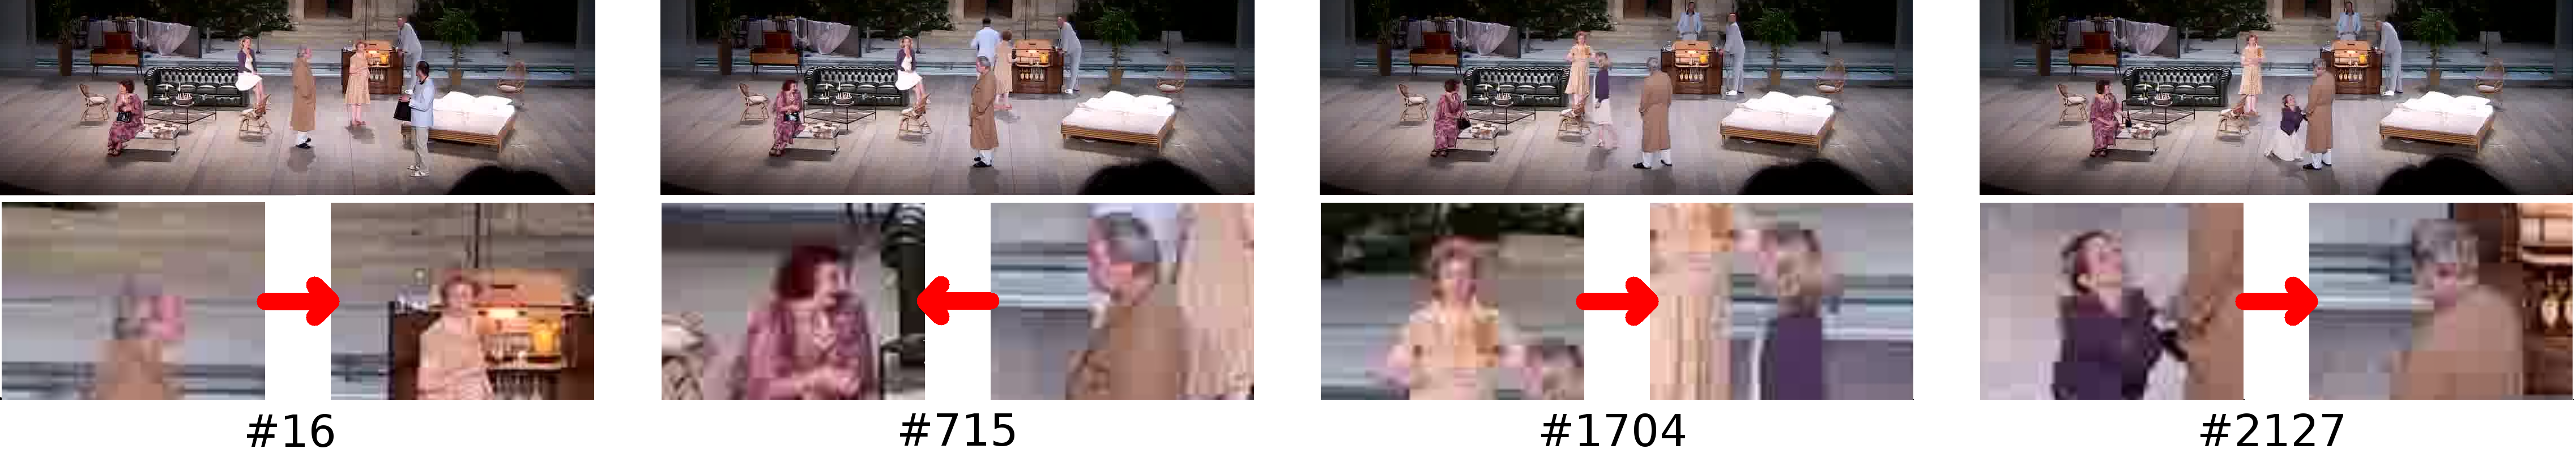
\includegraphics[width=\textwidth]{speakers2}
\caption{Reframing of the videos during dialogues.  Audio-to-text alignment temporally localizes the actors speaking and being spoken to. Video tracking  spatially localizes them on screen.  This figure displays the automatic reframing process obtained for several frames on the sequence $\mathcal{S}_4$. The arrows go from the speaker to the addressee.}
\label{fig_speaker}
\end{figure*}

Both the spatial and the temporal zoom lenses were assembled into 
an online  application using Web Components. The application is available at
%\url{http://spectacleenlignes.fr/hypervideo/}
\todo{anonymized URL}
and the implementation is  shared as open source. A~screenshot of the application can be seen in Figure~\ref{fig:screenshot}.

\begin{figure}[htb!]
  \centering
  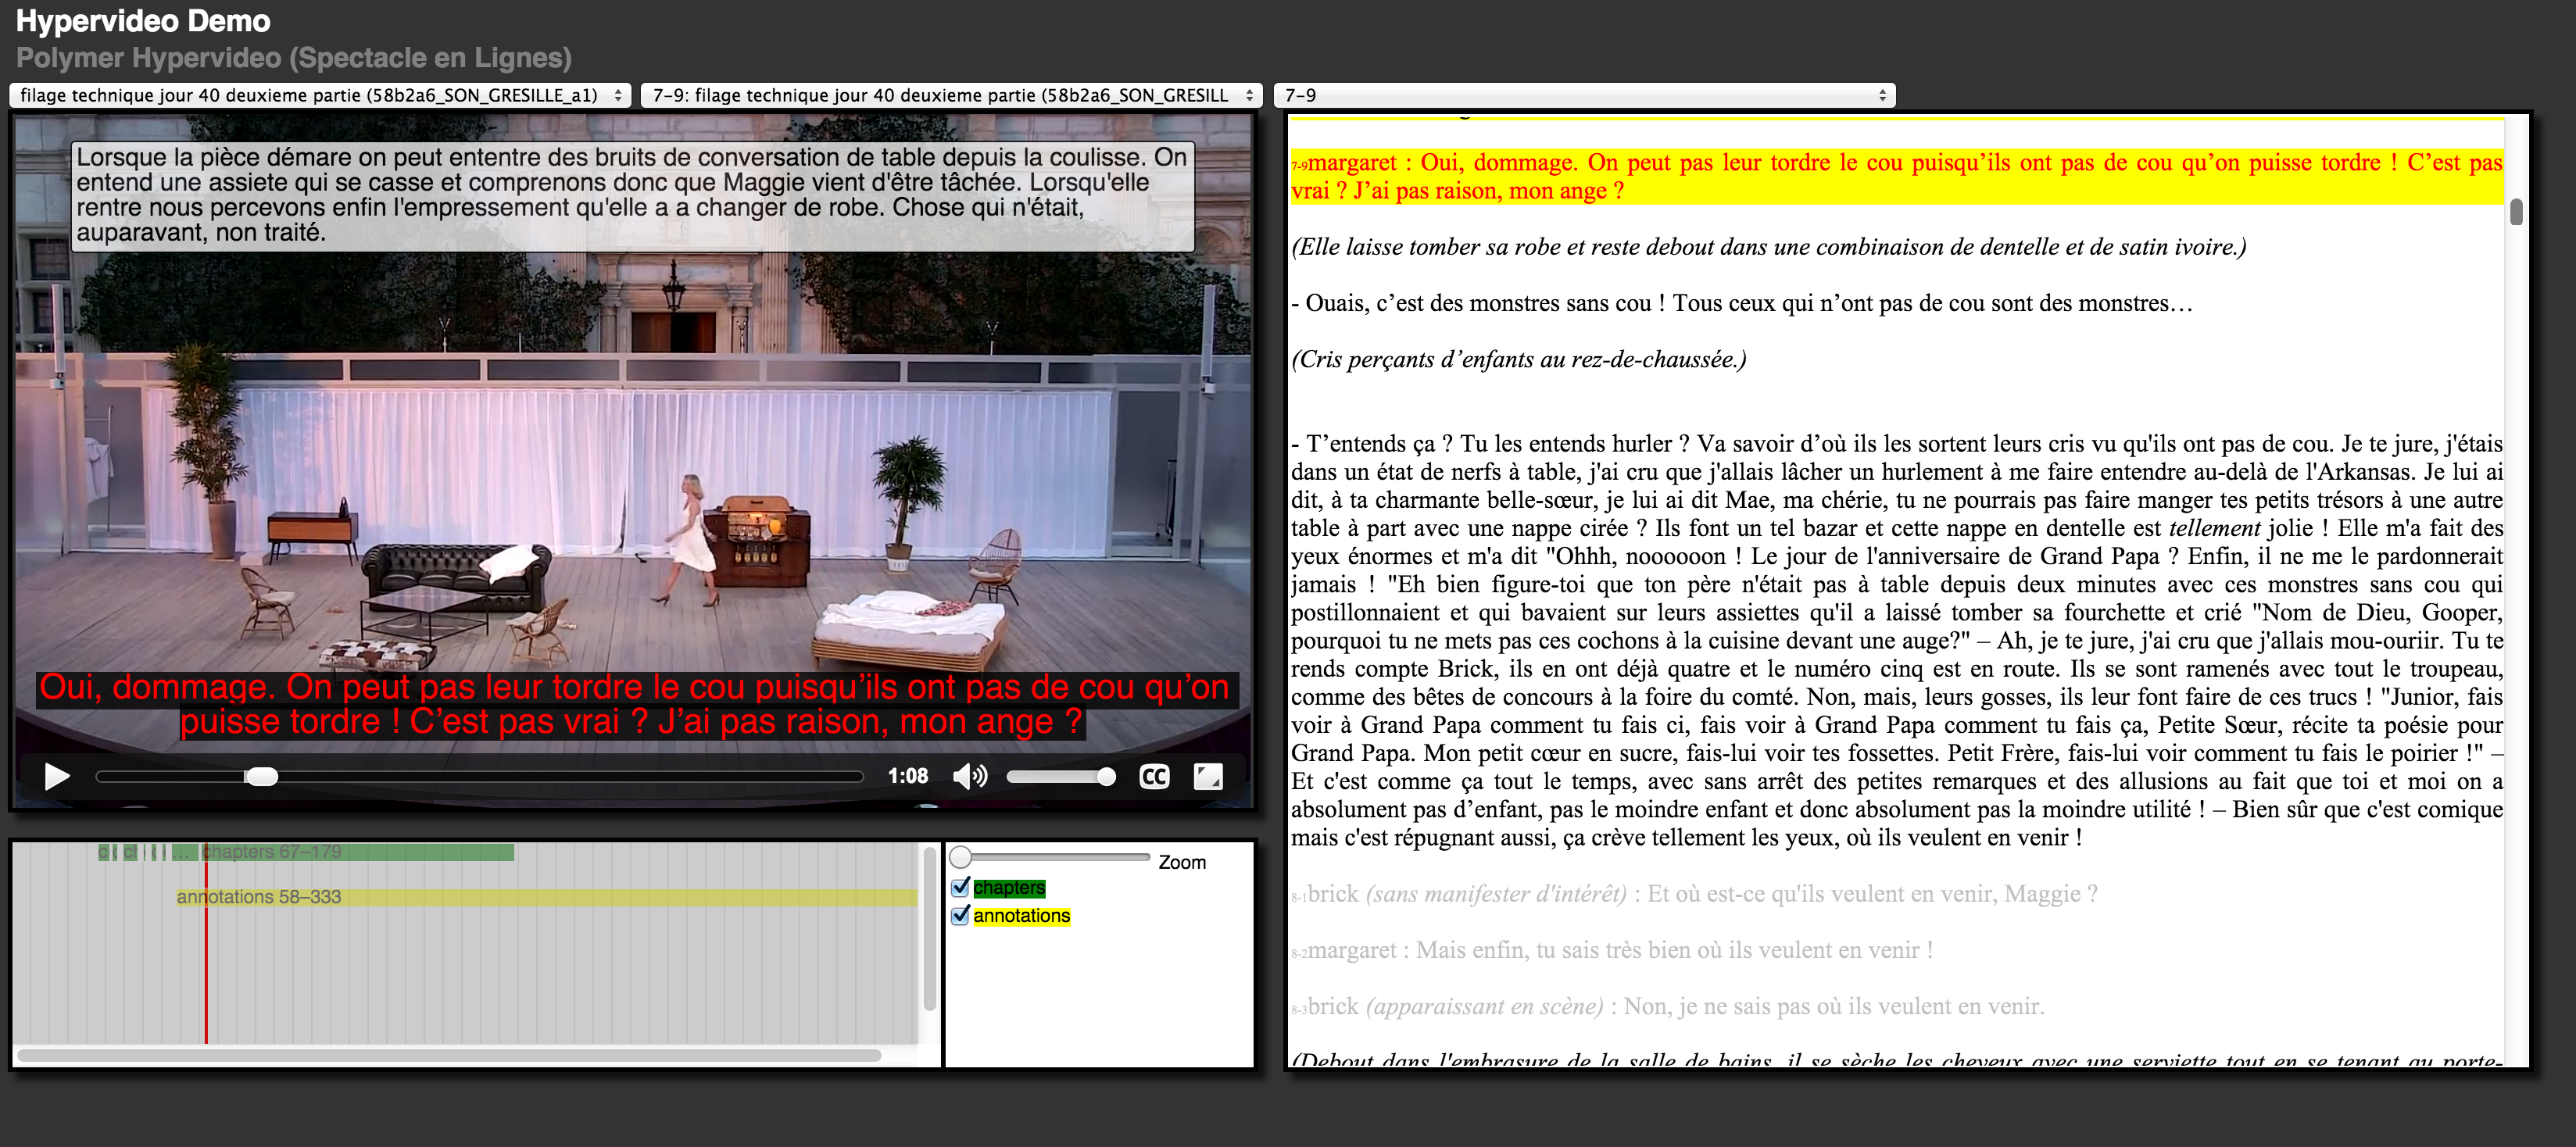
\includegraphics[width=0.95\linewidth]{screenshot}
  \caption{Generated hypervideo including subtitles, cue selectors, timeline, and connected play script
    showing a~rehearsal scene from day~40.}
  \label{fig:screenshot}
\end{figure}


% have a responsability in the design and the implementation of those conditions for ressources appropriation \cite{sauret2015}.

%\subsection{Experimental validation}
%\todo{The recordings have been evaluated subjectively by the actors, the director and her assistants?}
%\todo{A separate evaluation is being performed by film editors.}
%\todo{We can use Pascal Bouchez evaluation grids to assess the quality of the dataset?}


%%%%%%%%%%%%%%%%%%%%%%%%%%%
%\section{Limitations and Future  Work}
%\label{sec:limitations}


%\subsection{Mobile app for the creative crew} 
%\todo{Remarque BE: section à supprimer si besoin de place, mettre un petit quelque chose dans les futur work dessus
%NS: c'est la discussion qu'on a eu au dernier call, mais cette section est essentielle pour cette section Scenario et usage de l'archive, surtout dans le contexte d'une conférence Digital Heritage, où l'on montre les potentialités d'usage réelles, et non pas simplement des démonstrateurs hors-sol. C'est tout le travail de scénario qui a été fait dans ce projet et qui ne doit pas mis de côté, en particulier pour cette conférence. Je te renvoie à l'introduction de cette section qui réintroduit la démarche du projet, à savoir d'avoir imaginé une archive tout en réfléchissant à des scénarios d'usage.}
%
%A more complete scenario was designed to illustrate potential usage of the archive. In the context of the creative process itself, this scenario involves a mobile app that members of the crew could use to review, annotate and discuss the rehearsals along the direction process. Such an app would benefit from the complete workflow from video capture to video online publication and would provide the creative crew a excellent assistant to mark, search and archive the memory of the creative process. During the project, we developed the full user experience and interface into mock-ups (Figure~\ref{fig:mobileapp}).
%
%\begin{figure}[htb!]
%  \centering
%  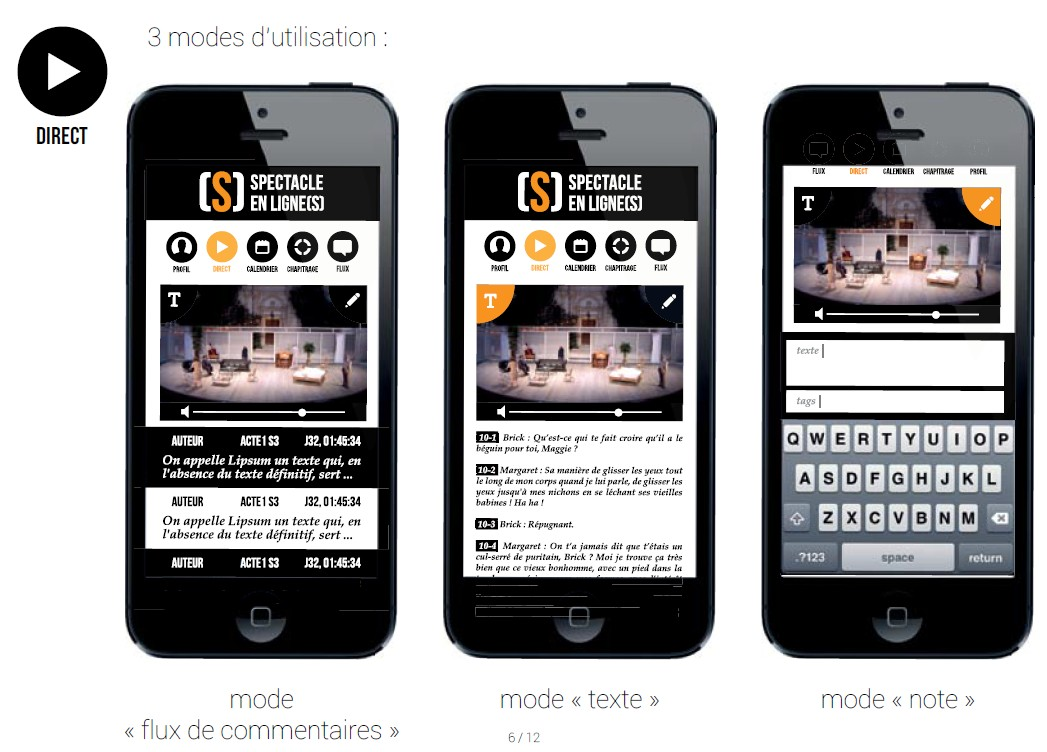
\includegraphics[width=\columnwidth]{mobileapp}
%  \caption{Mobile app: extracts of the design mock-ups}
%  \label{fig:mobileapp}
%\end{figure}
%
%
%This scenario reveals an interesting result in terms of digital heritage issue. In fact, it appears that digital archives meet the present needs of certain users whose objectives are not necessarily to augment the production of knowledge. Digital archive should therefore articulate freely with new communities of potential actors and users. One of the results of \emph{Spectacle en ligne(s)} is the demonstration that this empowerment of users with digital ressources must be accompanied by a set of technological conditions (an applicative platform for instance) and involvement of cultural institutions. \todo{RR: Nicolas, is this what you originally meant ?}


\subsection{Mobile app for the creative crew} 


During the production of the archive, the creative crew reacted quite positively to the experiment and expressed  interest in getting immediate feedback. While this had not been planned, we started designing mobile applications that they could tentatively use for \emph{(i)}~viewing the live feed being recorded on their smartphones and \emph{(ii)}~adding their own (signed) annotations and comments collaboratively.  While not fully implemented, this feature was presented to the directors and their collaborators as mock-ups (Figure~\ref{fig:mobileapp}). These mock-ups were generally well received and are likely candidates  as an addition to the existing system for future experiments. 

\begin{figure}[htb!]
  \centering
  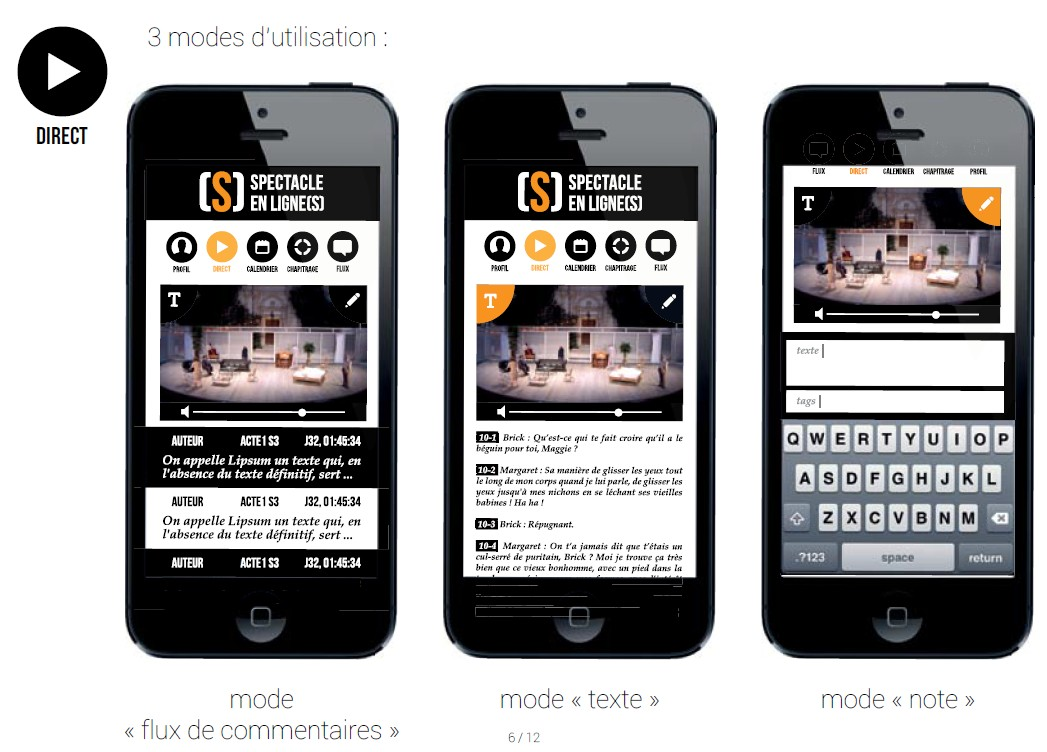
\includegraphics[width=\columnwidth]{mobileapp}
  \caption{Mobile app: extracts of the design mock-ups}
  \label{fig:mobileapp}
\end{figure}


 


%%%%%%%%%%%%%%%%%%%%%%%%%%%
\section{Conclusion}
\label{sec:conclusion}

The research described in this paper was accomplished over a~period of two years 
in close collaboration with the directors of the two documented productions and was 
contrary to all expectations well received by the performers and technical crew. Filming the rehearsals
from the director's point-of-view was a~key element for this positive response. In future work,
we would like to increase the video resolution of the recordings to 4K in order to better exploit
the capabilities of our virtual zoom lens; and to experiment with stereoscopic 3D and 360\degree~panoramic video
which would allow to include reverse shots of the directors and their assistants, which are currently not recorded.

It is our hope that this archive illustrates the cultural heritage of the performing arts from a~novel and 
interesting perspective. Audio, video and Web technologies were used to augment
the raw video with fully integrated metadata and spatio-temporal zooming capabilities,
which proved invaluable to make the archive attractive to researchers and amateurs.
Nevertheless, the resulting archive is overwhelming and more focused future work is needed to 
better measure its impact and usefulness in the digital humanities. 


%\todo{Paragraph on legal aspects? NS> why not in the limitations instead} 
%Future work is needed to fully evaluate the zooming feature in the light of  the theory  of spectatorship, 
%which surveys the audience's visuomotor behavior  during a performance~\cite{Bennett97}. 

%M\todo{Expand more on promising directions for future research, including the notation of theater,
% copyright protection for stage directions, the possibility of a depot legal, etc.}

% conference papers do not normally have an appendix

% use section* for acknowledgement
%\section*{Acknowledgment}
%\todo{The authors would like to thank...}
% \todo{Balance reference columns}




% trigger a \newpage just before the given reference
% number - used to balance the columns on the last page
% adjust value as needed - may need to be readjusted if
% the document is modified later
%\IEEEtriggeratref{8}
% The "triggered" command can be changed if desired:
%\IEEEtriggercmd{\enlargethispage{-5in}}

% references section
%\nocite{*}


% can use a bibliography generated by BibTeX as a .bbl file
% BibTeX documentation can be easily obtained at:
% http://www.ctan.org/tex-archive/biblio/bibtex/contrib/doc/
% The IEEEtran BibTeX style support page is at:
% http://www.michaelshell.org/tex/ieeetran/bibtex/
\bibliographystyle{IEEEtran}
% argument is your BibTeX string definitions and bibliography database(s)
\bibliography{rehearsals}




% that's all folks
\end{document}
